% !TEX root = ../Thesis.tex
\chapter{Muon Tagging in a boosted \ttbar\ environment} \label{sec:boosted_study}

The large center-of-mass energies at which collisions occur at the LHC allows for the production of very high mass particles. Several Beyond the SM (BSM) theories predict the existence of high mass particles which decay primarily top quark pairs.
An example of hypothetical model which predict high mass \ttbar\ resonances is the topcolor assisted technicolor model (TC2), which predicts the existence of a leptophobic \Zprime\ boson. The resultant top quark pair provides a well understood probe to search for such hypothetical particles. 

The \Zprime\ could potentially have a mass on the order of several TeV. As a result their decay product would be produced in the detector with very large momentum. These top quarks are said to be boosted. In terms of the subsequent top decay, the resultant bottom quark and \W\ boson are expected to emerge in a collimated cone. The events thus appear as two large back-to-back jets. If the \W\ decays leptonically, the \W\ lepton is expected to lie very close to or within the $b$-jet. If the \W\ decays hadronically all three jets will appear to merge into a single 'fat' jet.

In this chapter the results of a feasibility study conducted to determine the viability of using the \xsm\ tagger to tag \W\ muons from boosted top-quark decays is presented and discussed. Note that this is in contrast to the cross-section analysis detailed in a previous chapter where the muon tagged came from the semileptonic decay of $b$-quarks. The boost is expected to be related to the mass of the \Zprime\ produced, so a higher mass \Zprime\ would decay into more collimated jets. The environment that results is thus very similar to that of a semileptonic $b$-decay, a muon buried inside of a $b$-jet.

No evidence for such a resonance has been observed and limits have been placed on the production rate of these resonance for various benchmark models. A leptophobic topcolor \Zprime\ of mass less than 1.74 TeV has been excluded using 4.7 fb$^{-1}$ of $pp$ collision data collected by ATLAS with a center-of-mass energy $\sqrt{s}=7$ TeV \cite{Boosted:ATLASExclusion7TeV}. Additionally a more recent analysis using 14.3 fb$^{-1}$ of $\sqrt{s}=8$ TeV data collected at ATLAS excluded a \Zprime\ with a mass less than 1.8 TeV at $95\%$ confidence level \cite{Boosted:ATLASExclusion8TeV}.  The analysis detailed here is based on the 7 TeV analysis. Similar analyses performed with data collected by CMS have excluded \Zprime\ candidates for similar benchmark models \cite{Boosted:CMSSearch7TeVDilepton,Boosted:CMSSearchAnomalous,Boosted:CMSSearch8TeV}. 

The performance of SMT is compared to the contemporary method for selecting muons known as mini-isolation. In addition a short performance study to determine the viability of using SMT to tag $b$-jets in boosted top events is also presented. Firstly, a short examination of the topology of a boosted event is presented.

\section{Boosted event topology}

In order to perform an effective feasibility study, it is important to understand the signature left by boosted events in the detector. There are certain expectations regarding the momentum distribution of the various product particles from the decay of the top as well as their angular separation. As with the cross-section analysis presented in Chapter~\ref{sec:cross_section}, this study focuses on the semileptonic decays of top quark pairs

It is expected for events where the momentum of the top quarks higher to exhibit stronger collimation between the \W\ muon and the $b$-quark. This results in a situation very similar to that exploited for muon tagging in Section~\ref{sec:cross_section} where a muon from the semileptonic decay of a $b$-quark emerges from within the $b$-jet. Fig.~\ref{fig:SimpleAngularDiagrams} illustrates the similarity of both scenarios. It is thus possible to use the \xsm-tagger\footnote{As signal muons are very hard, the tagger is now refered to as the \xsm tagger not soft muon tagger to reflect this difference} to tag \W\ muons in boosted events. As the tagger is designed to work in energetically "busy" sectors of the detector, it is ideally suited to probe highly boosted events where the decay products are collimated.

\begin{figure}[t]
  \begin{subfigure}[b]{0.45\textwidth}
    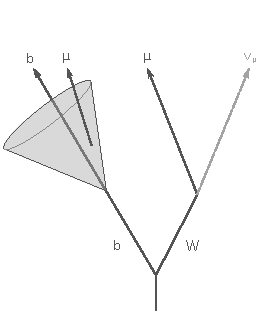
\includegraphics[width=\textwidth]{PartBoosted/Plots/NonBoosted.pdf}
    \caption{Non-boosted event} \label{fig:NonBoostedDiagram}
  \end{subfigure}%
  ~ 
  \begin{subfigure}[b]{0.45\textwidth}
    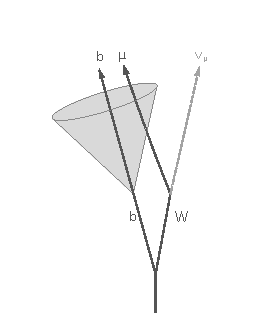
\includegraphics[width=\textwidth]{PartBoosted/Plots/Boosted.pdf}
    \caption{Boosted event} \label{fig:BoostedDiagram}
  \end{subfigure}
  \caption{This figure shows a simple diagram for the possible configuration of final-state objects in a (a) boosted and (b) non-boosted events. Note that in both cases a muon is embedded within the $b$-jet} \label{fig:SimpleAngularDiagrams}

\end{figure}

As can be seen from Fig.~\ref{fig:ExampleCollimation} the increase in boost does result in the \W\ muon and $b$-quark emerging closer. Note that the fraction of events below the SMT requirement of $\Delta R(\mu,jet)<0.5$ increases with increased top-quark \pt. Additionally Fig.~\ref{fig:ExampleBoost} shows that the top \pt\ distribution peaks at just below half of the mass of the \Zprime\ boson, thus the large portion of the candidate muons in the sample will pass the aforementioned separation requirement. The decay products of the top quark appear to emerge primarily back to back as seen in Fig.~\ref{fig:ExampleBackToBack}.

\begin{figure}[t]
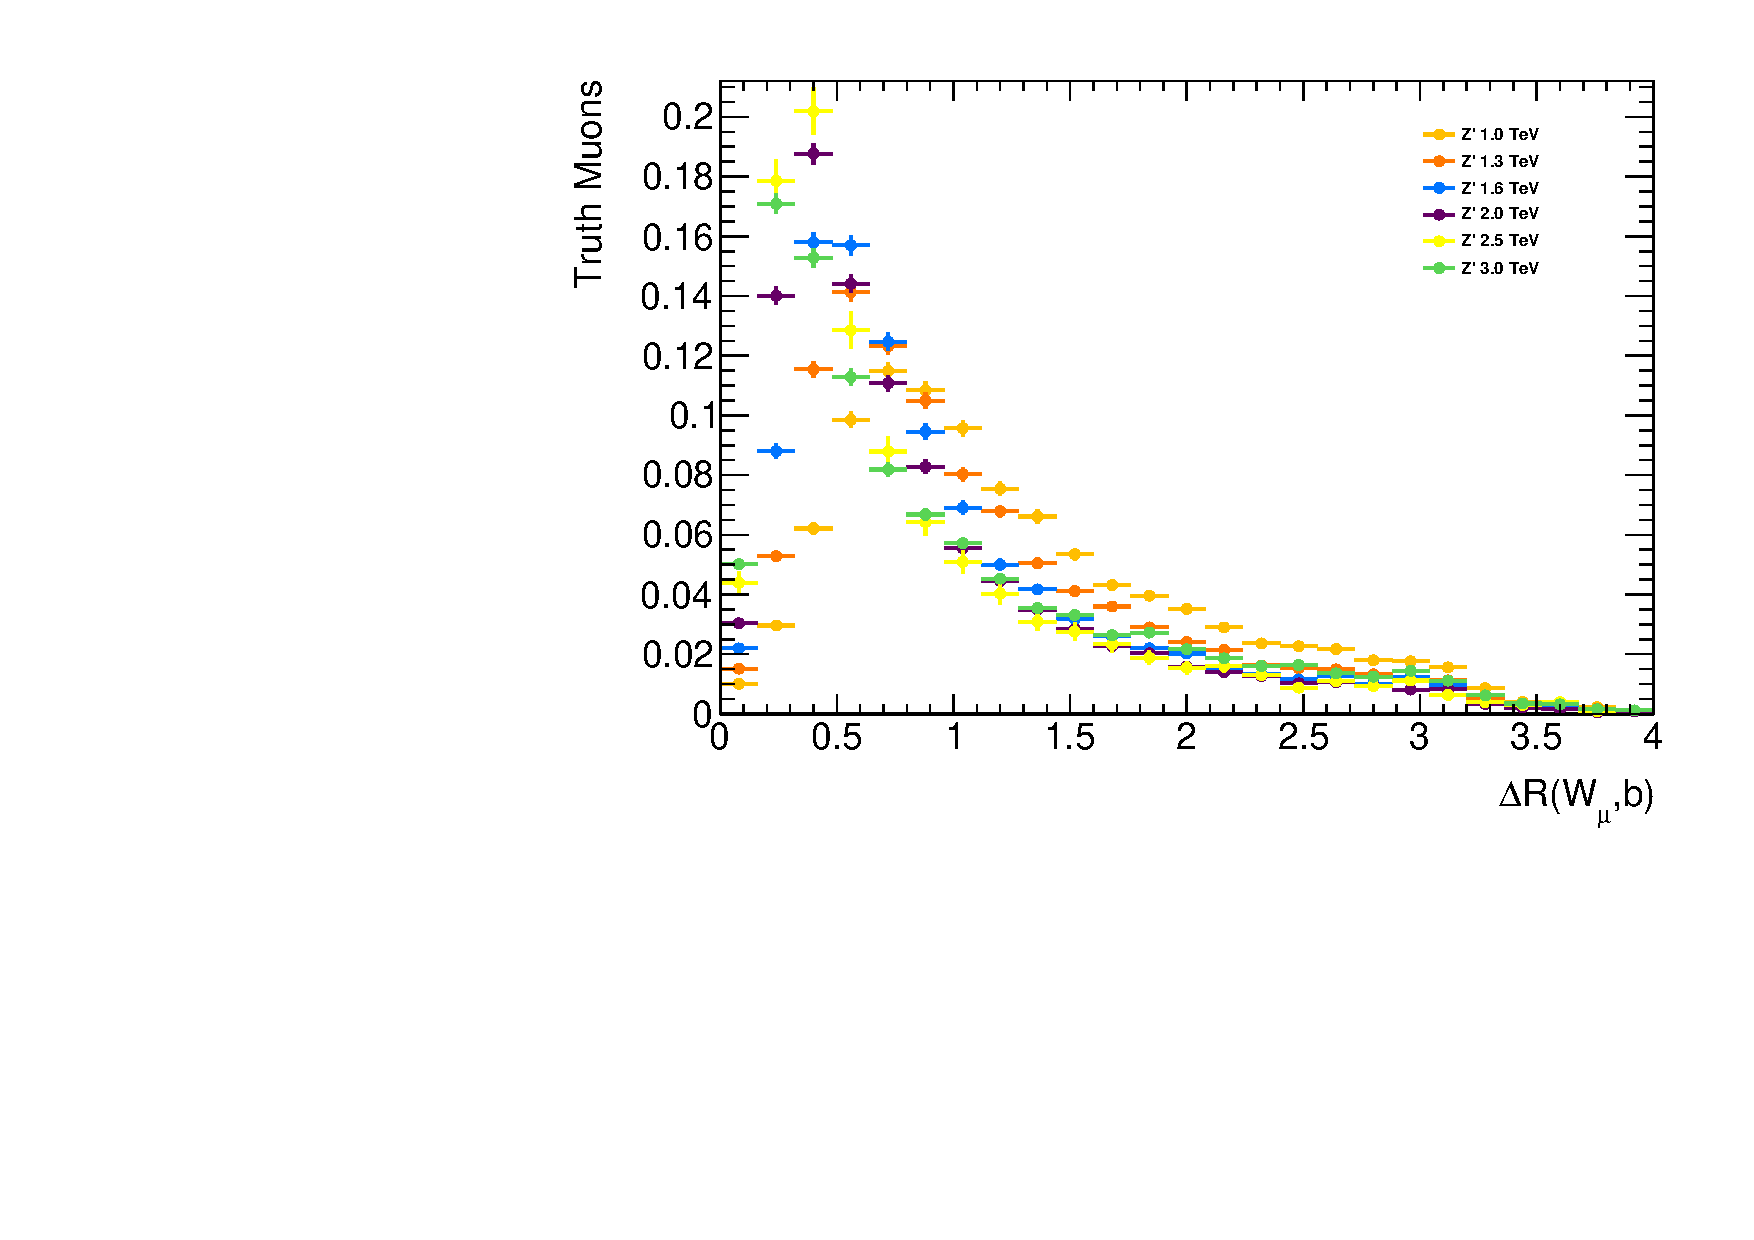
\includegraphics[width=\textwidth]{PartBoosted/Plots/h_trmu_b_dr.pdf}
\caption{The angular separation ($\Delta R$) between the truth \W\ muon and the corresponding $b$-quark for all examined \Zprime\ mass points.} \label{fig:ExampleCollimation}
\end{figure}

\begin{figure}[t]
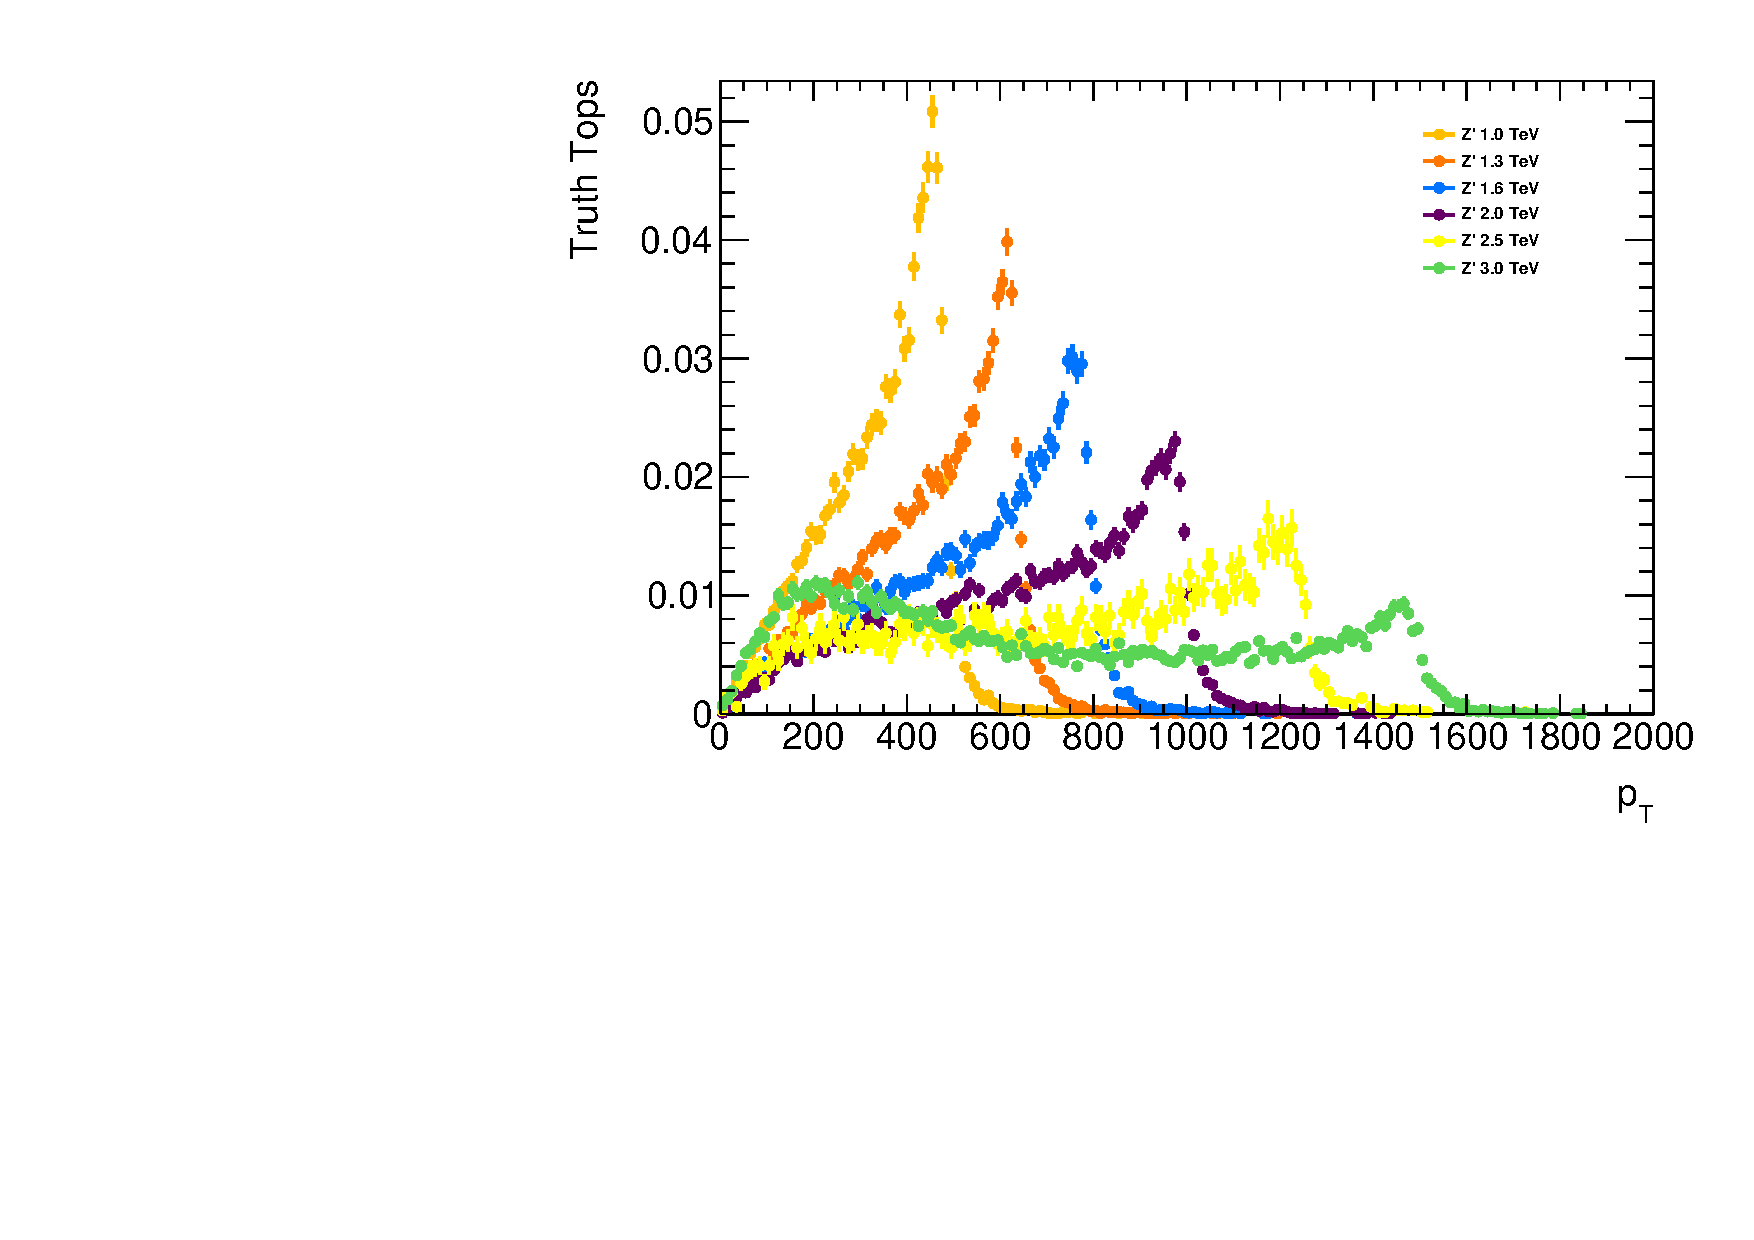
\includegraphics[width=\textwidth]{PartBoosted/Plots/h_trtop_pt.pdf}
\caption{The transverse momentum of the top/anti-top quarks in the event for all examined \Zprime\ mass points.} \label{fig:ExampleBoost}
\end{figure}

\begin{figure}[t]
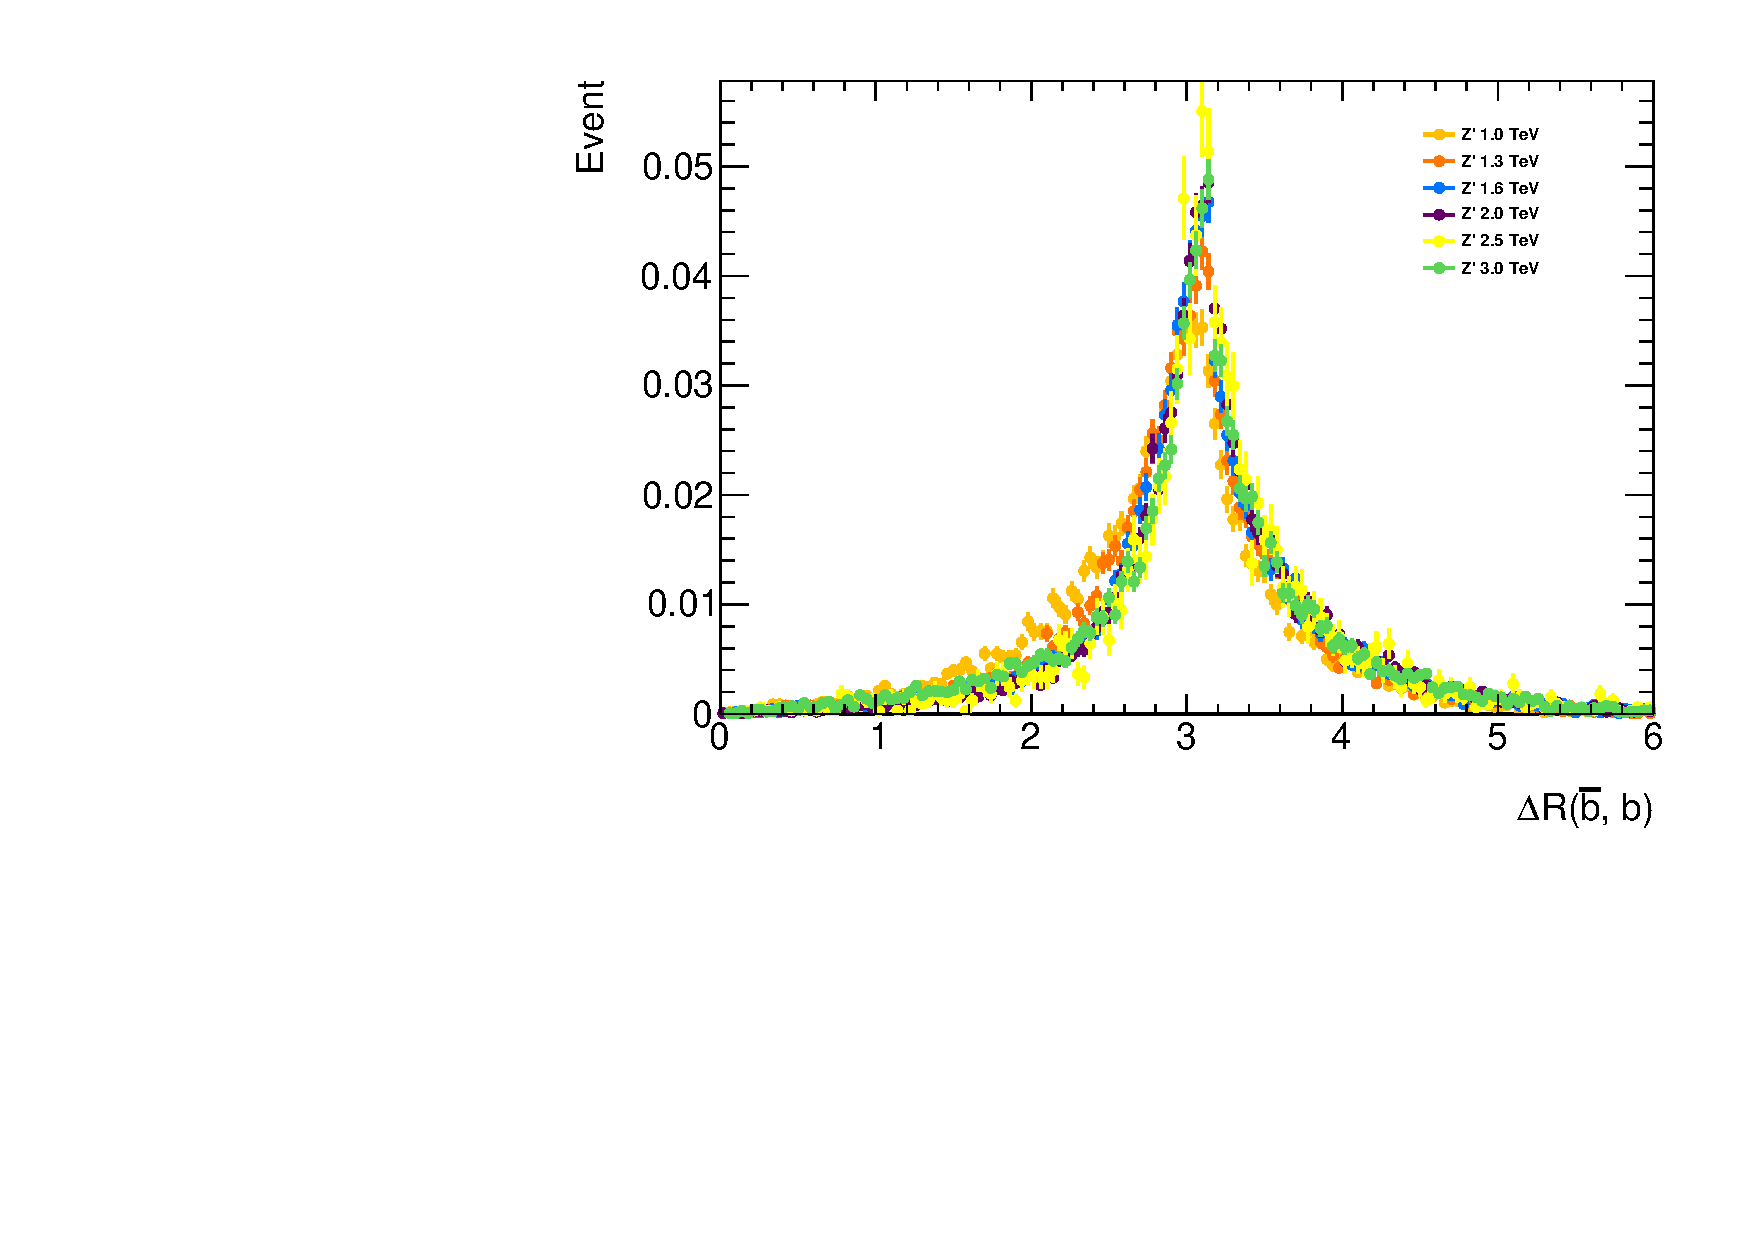
\includegraphics[width=\textwidth]{PartBoosted/Plots/h_b_bbar_dr.pdf}
\caption{The angular separation ($\Delta R$) between the $b$ and $\overline{b}$ in the event for all examined \Zprime\ mass points.} \label{fig:ExampleBackToBack}
\end{figure}

\section{Samples and muon selection}

This measurement is based on simulated data generated for a \Zprime\ with a mass of 1.0, 1.3, 1.6, 2.0, 2.5 and 3.0 TeV. All Monte Carlo (MC) samples were generated using \textsc{PYTHIA} with CTEQ6LI PDFs. The width of the generated \Zprime\ is $3\%$ of the mass. 

\section{Signal muon selection}

\subsection{Muon selection}
The nominal muon object selection includes an isolation requirement, which normally removes events where the signal lepton is found in a region of the calorimeter with large amounts of activity. Cutting on the amount of energy deposited in the calorimeter around the lepton is an example of one such requirement. Such a cut forms part of the object selection used in the top cross-section measurement described in Part~\ref{prt:Calibration}.

However, as described a priori, boosted top events result in large collimated jets which include the products of the two top quarks. Thus the signal lepton can emerge within the cone of the reconstructed jet from the $b$-quark. 

Note that the muon is not required to be isolated, instead the muon is tagged by the \xsm\ tagger. Selecting isolated muons would reduce significantly the number of muons available for tagging. Additionally, as explained a priori, events which exhibit stronger collimation are more likely to emerge from particles with higher masses. By requesting the muons be isolated, the ability to probe those higher mass events is diminished.

Another candidate to replace the traditional isolation selection is the so-called mini-isolation. This variable takes into account the strong collimation of the top products with increasing boost. Mini-isolation is defined as the sum of the measured transverse momenta of all tracks in a cone of size of size $\Delta R=k_{T}/p_{T}^{\ell}$ around the lepton, where $k_T$ is an adjustable scale and $p_{T}^{\ell}$ is the momentum of the lepton in question. This is known as the absolute mini-isolation. This study uses the relative mini-isolation where the absolute value is scaled by the momentum of the lepton ($MI/p_{T}^{\ell}$).

In this analysis the performance of the \xsm\ tagger is measured against mini-isolation using a $k_{T}=10$ and a lepton is deemed isolated if the $p_{T}$ in the MI cone is less than $5\%$ that of the lepton. The Muon Tagger operates with the same selection as used in Part~\ref{prt:Calibration}, the cuts are $|z_{0}|<3.0\textrm{ mm}$, $|d_{0}|<3.0\textrm{ mm}$ and finally $\xsd<3.2$.

Thus two separate selections are applied, one for for mini-isolation and one for SMT. Note that both methodologies have different muon reconstruction criteria, these are detailed in Table~\ref{tab:BoostedReconstruction}.

\begin{table}[th!]
  \centering
  \caption{Muon reconstruction selection used by Mini-Isolation and by Muon Tagging} \label{tab:BoostedReconstruction}
  \begin{tabular}{c|c}
  \hline
  Mini-Isolation & Muon-Tagging \\ \hline \hline
  \multicolumn{2}{c}{MCP Cuts} \\
  \multicolumn{2}{c}{$\pt>20\textrm{ GeV}$} \\
  \multicolumn{2}{c}{$|\eta|<2.5$} \\ \hline
  MUID & STACO \\ \hline
  $z_{0}<3.0\textrm{ mm}$ & Is Combined Muon \\ \hline
  IsEM Tight & \\ \hline
  \end{tabular}
\end{table}

\begin{figure}[t]
\begin{subfigure}{0.49\linewidth}
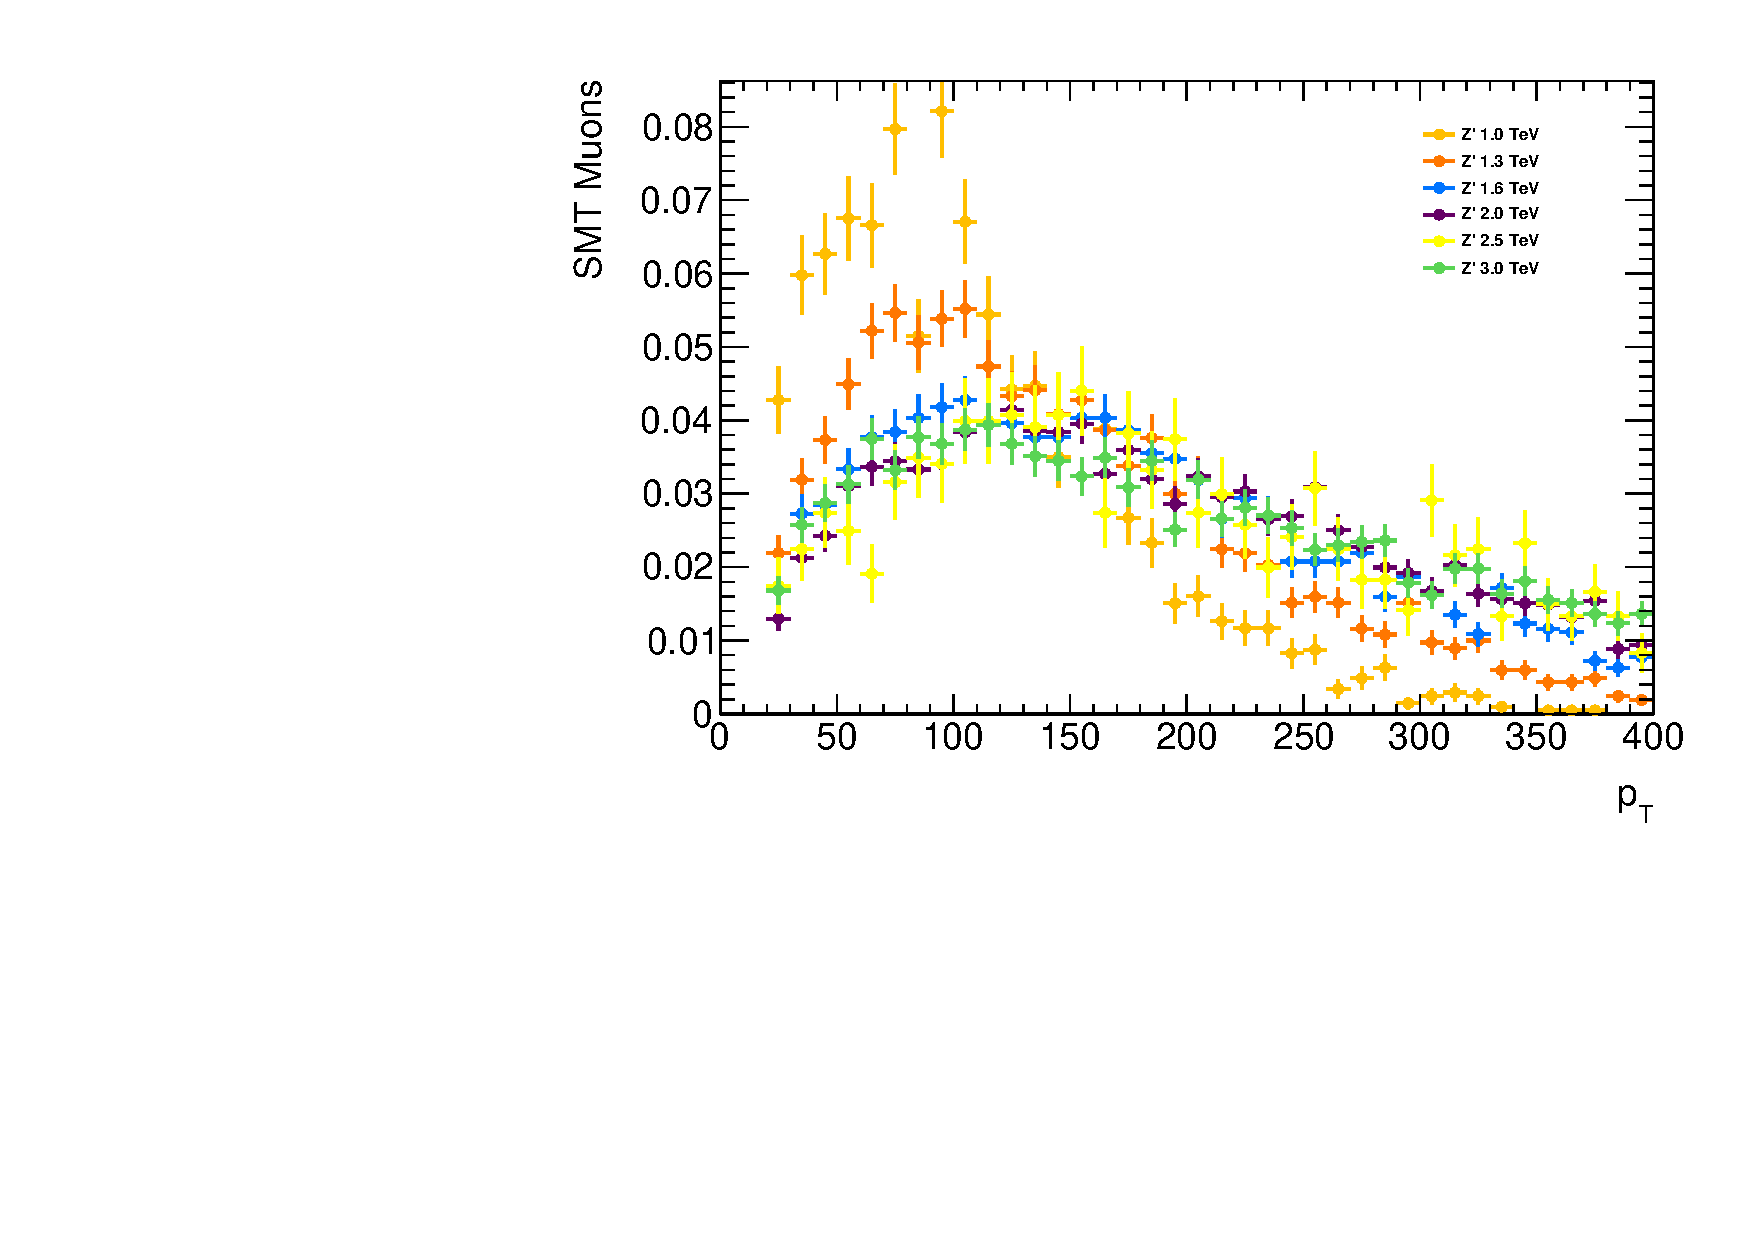
\includegraphics[width=\textwidth]{PartBoosted/Plots/h_smt_pt.pdf}
\end{subfigure}
~
\begin{subfigure}{0.49\linewidth}
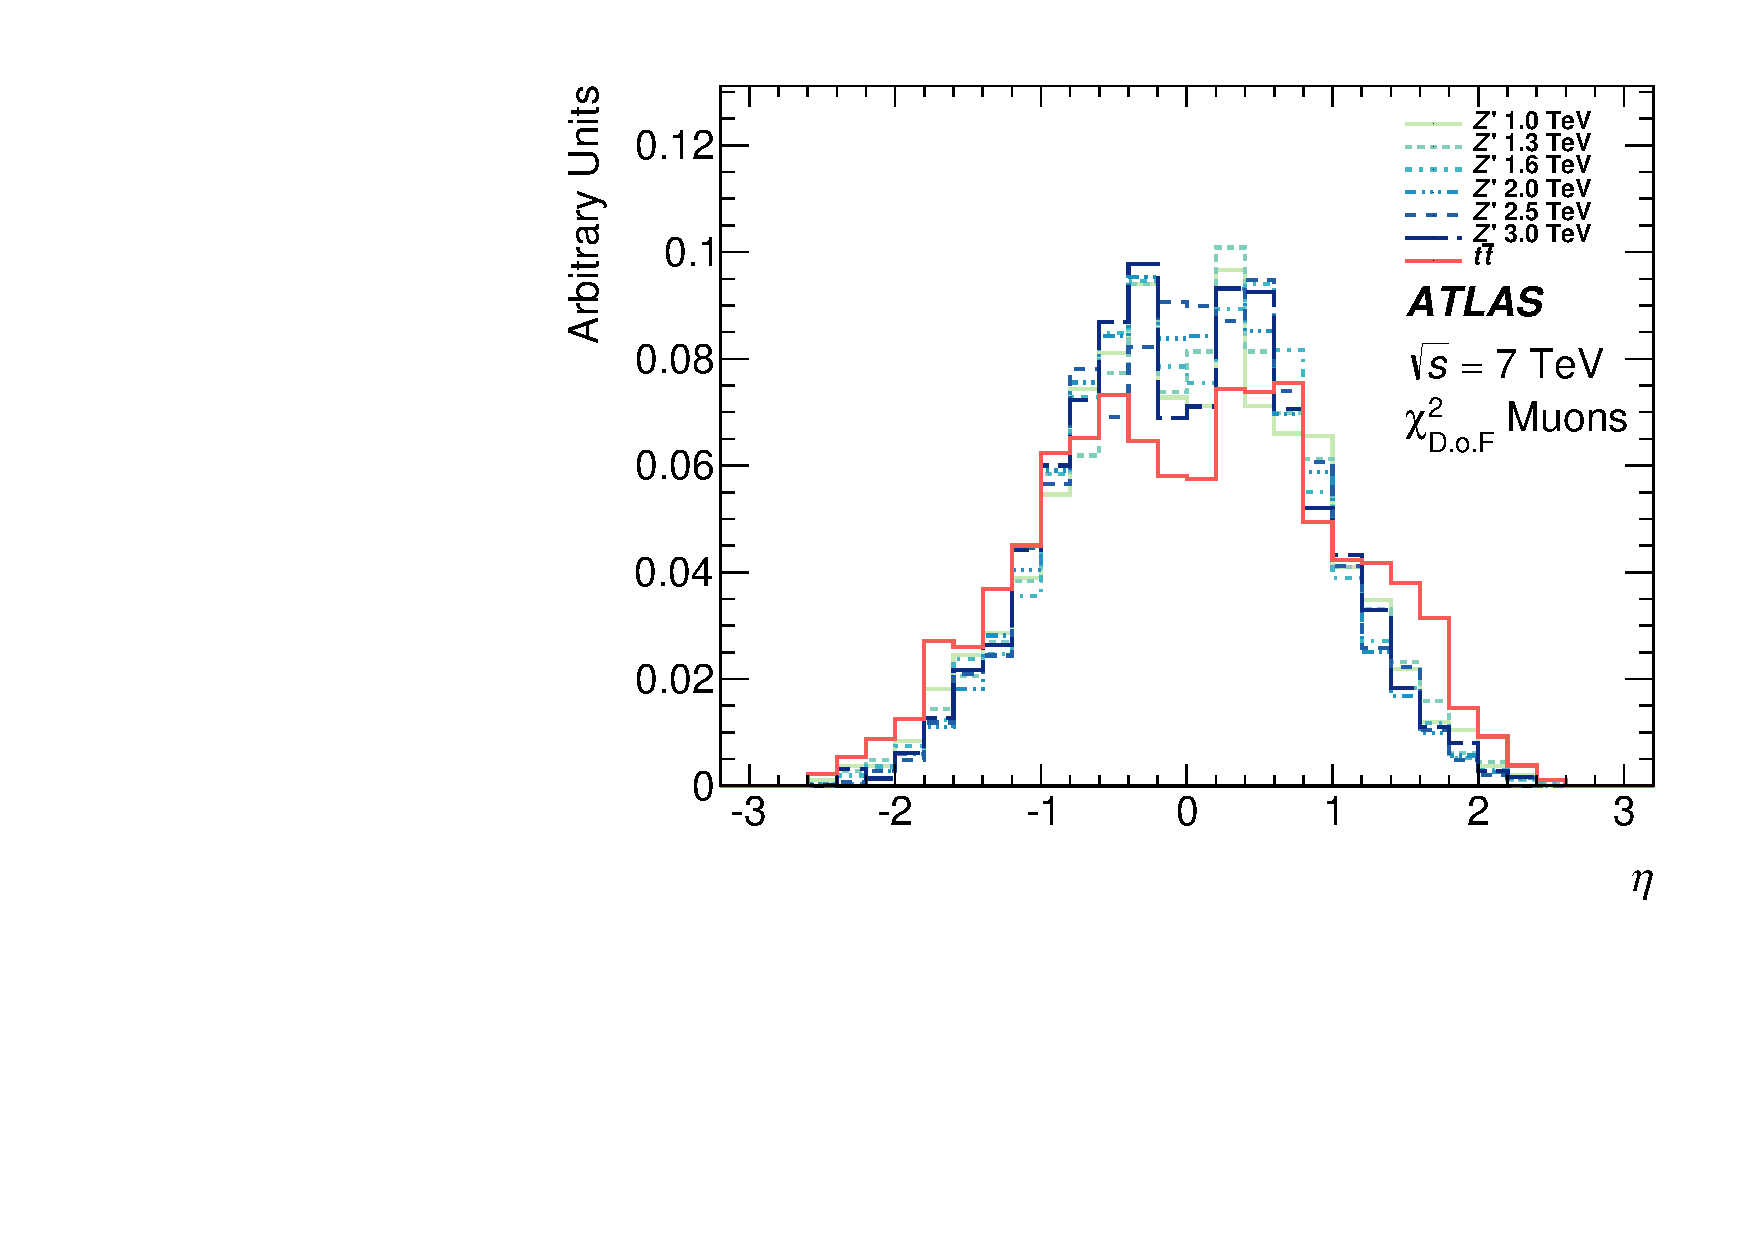
\includegraphics[width=\textwidth]{PartBoosted/Plots/h_smt_eta.pdf}
\end{subfigure}

\begin{subfigure}{0.49\linewidth}
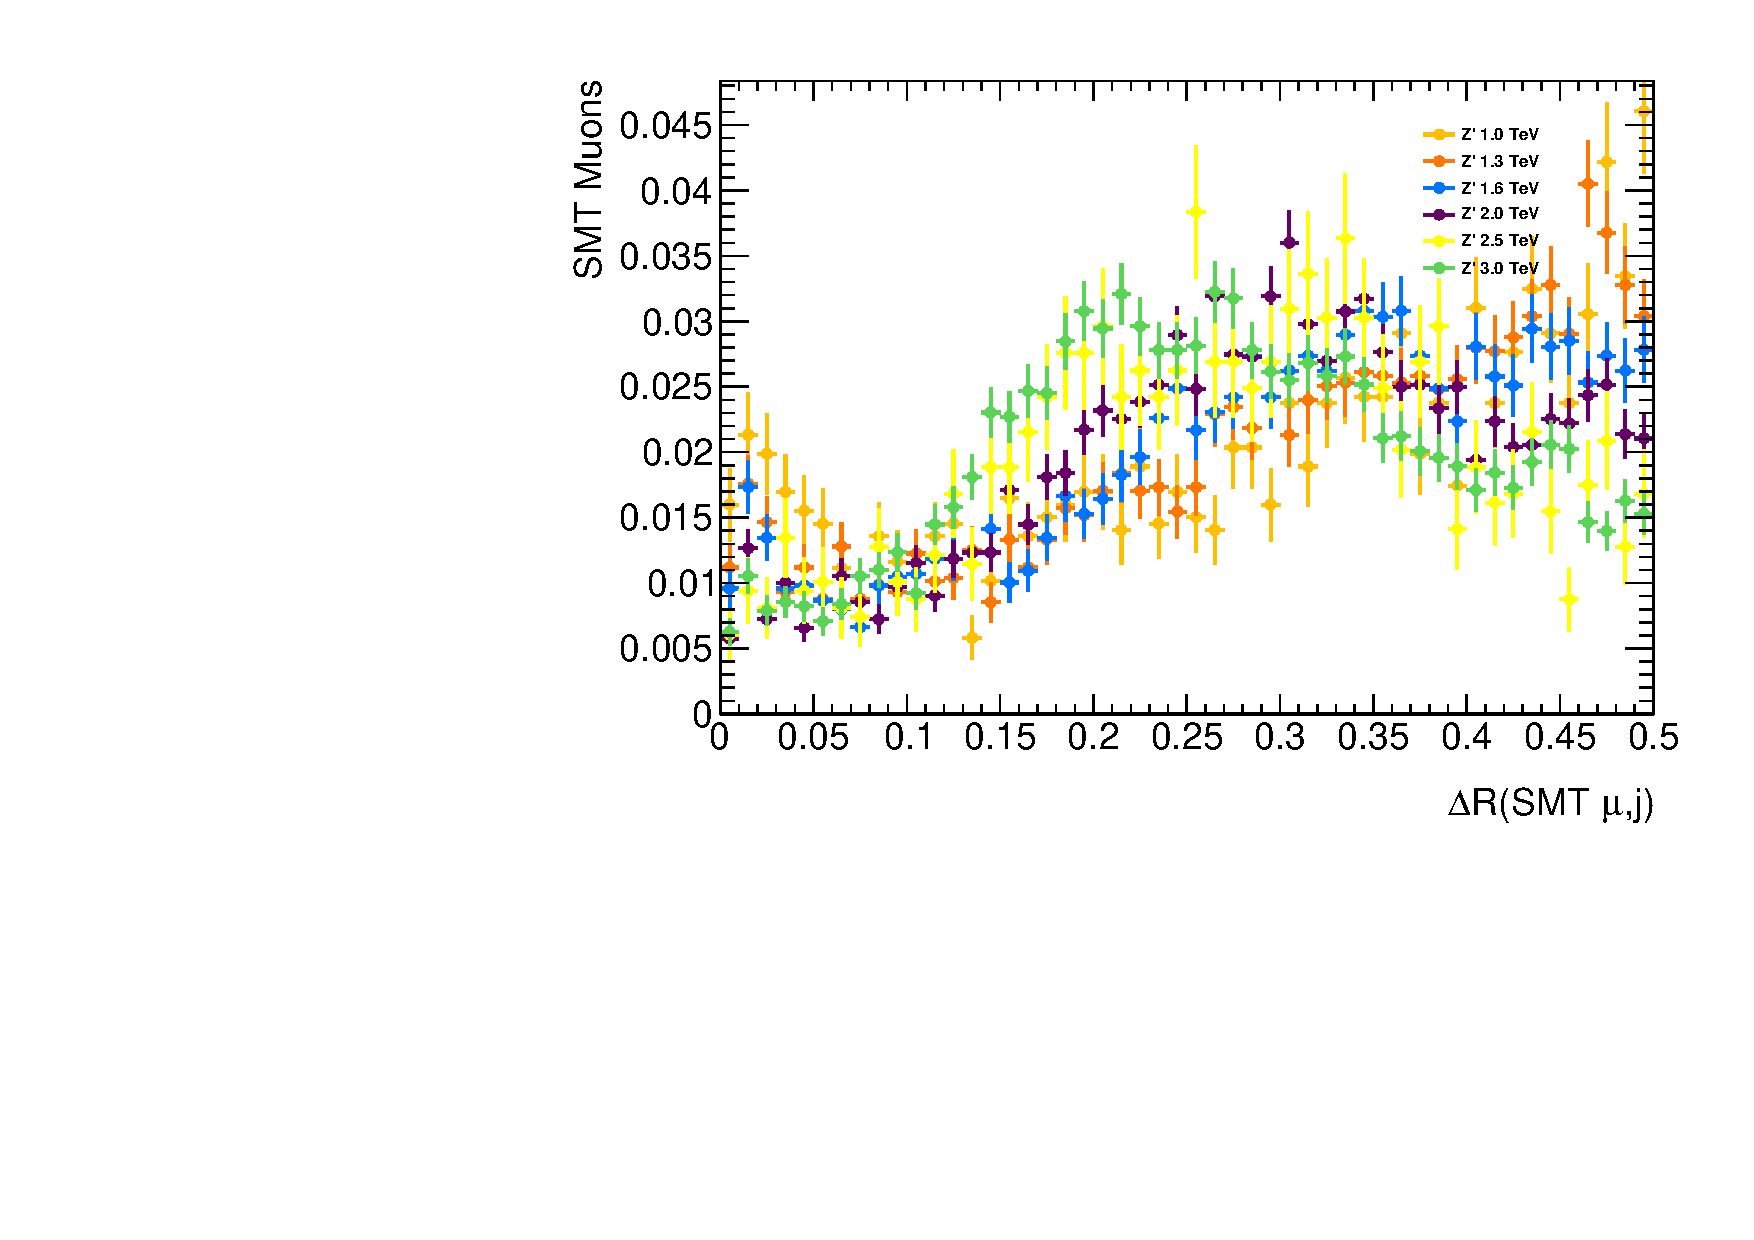
\includegraphics[width=\textwidth]{PartBoosted/Plots/h_smt_jet_dr.pdf}
\end{subfigure}
~
\begin{subfigure}{0.49\linewidth}
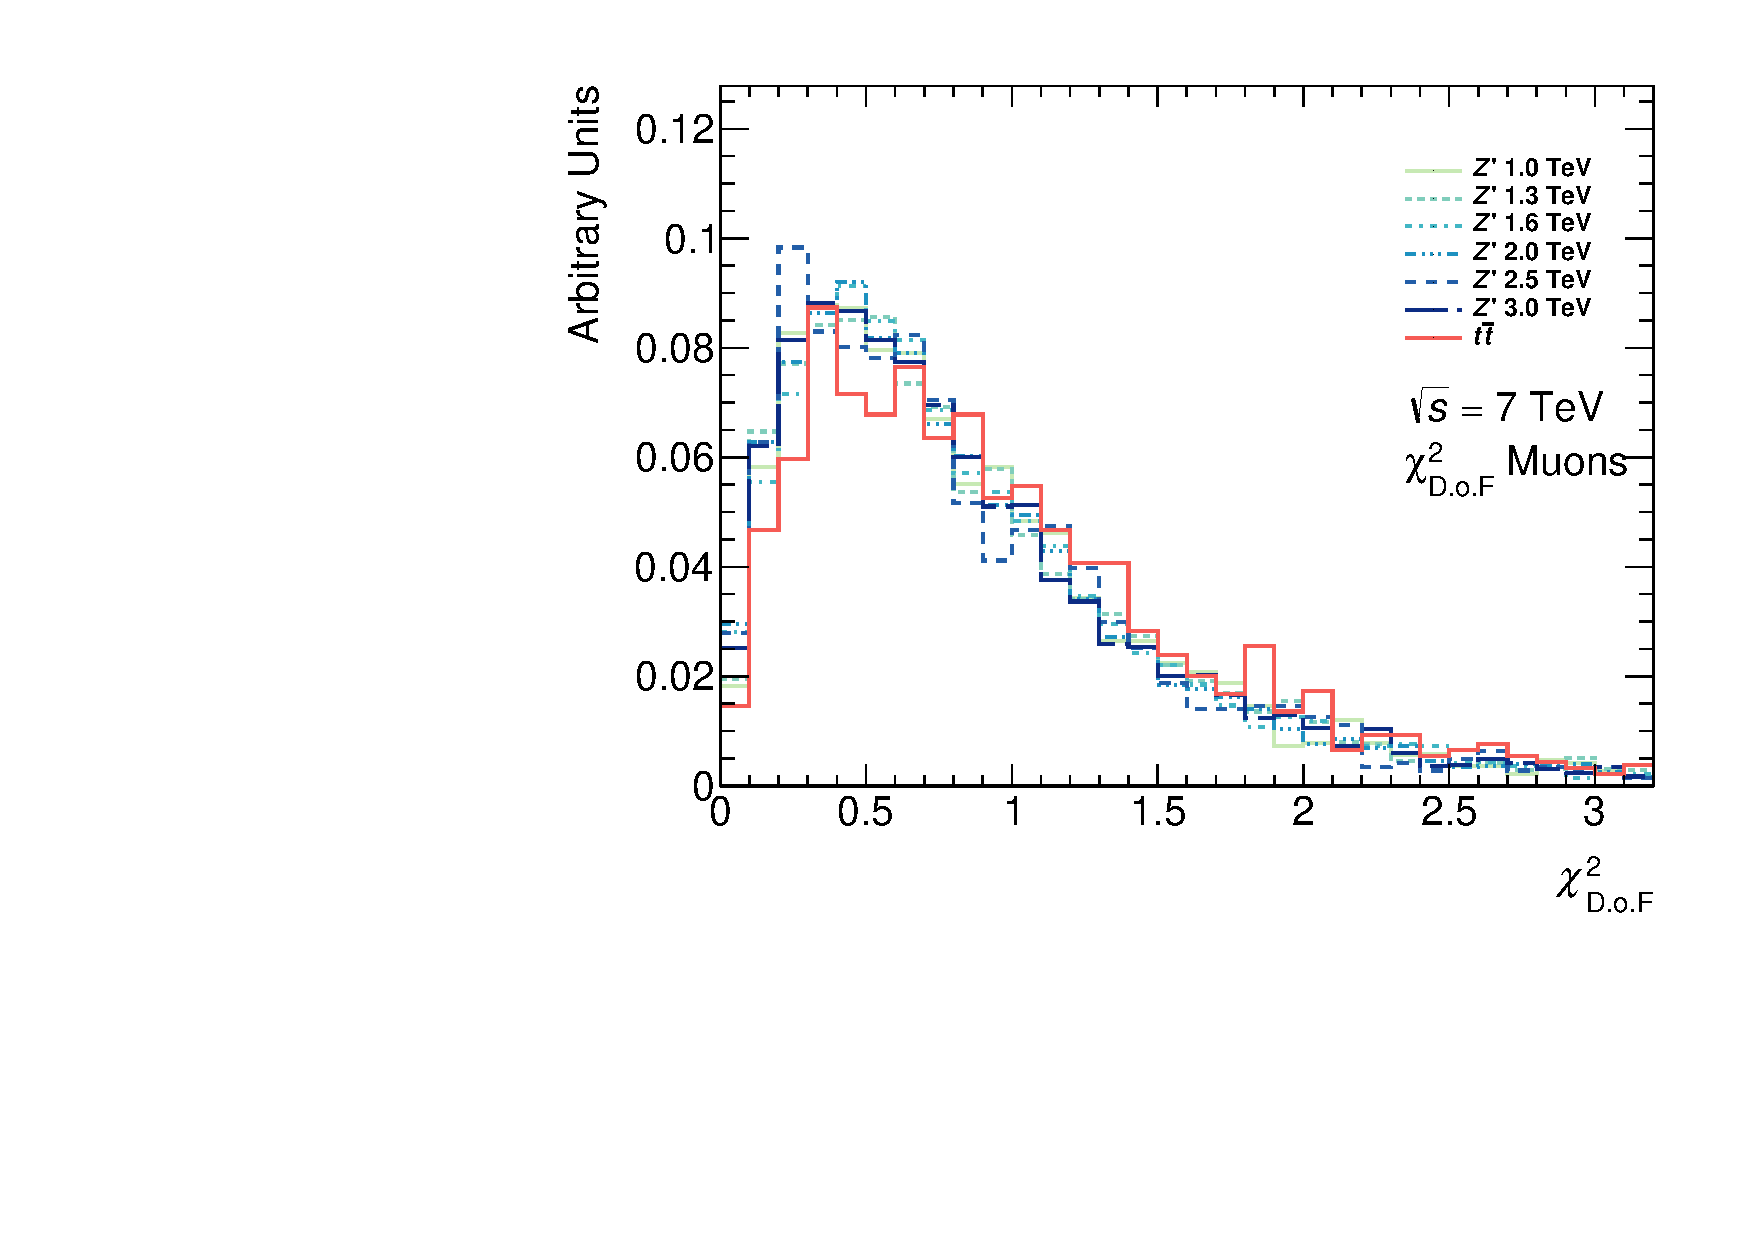
\includegraphics[width=\textwidth]{PartBoosted/Plots/h_smt_chi2.pdf}
\end{subfigure}

\caption{This figure shows the distribution of (a) transverse momentum and (b) pseudo-rapidity of muons which pass the SMT selection, the (c) angular separation between those muons and the nearest jet in th event and (d) the \xsm\ used in the selection for all tested \Zprime\ mass points.} \label{fig:BoostedControlMI10}
\end{figure}
\begin{figure}[t]
\begin{subfigure}{0.49\linewidth}
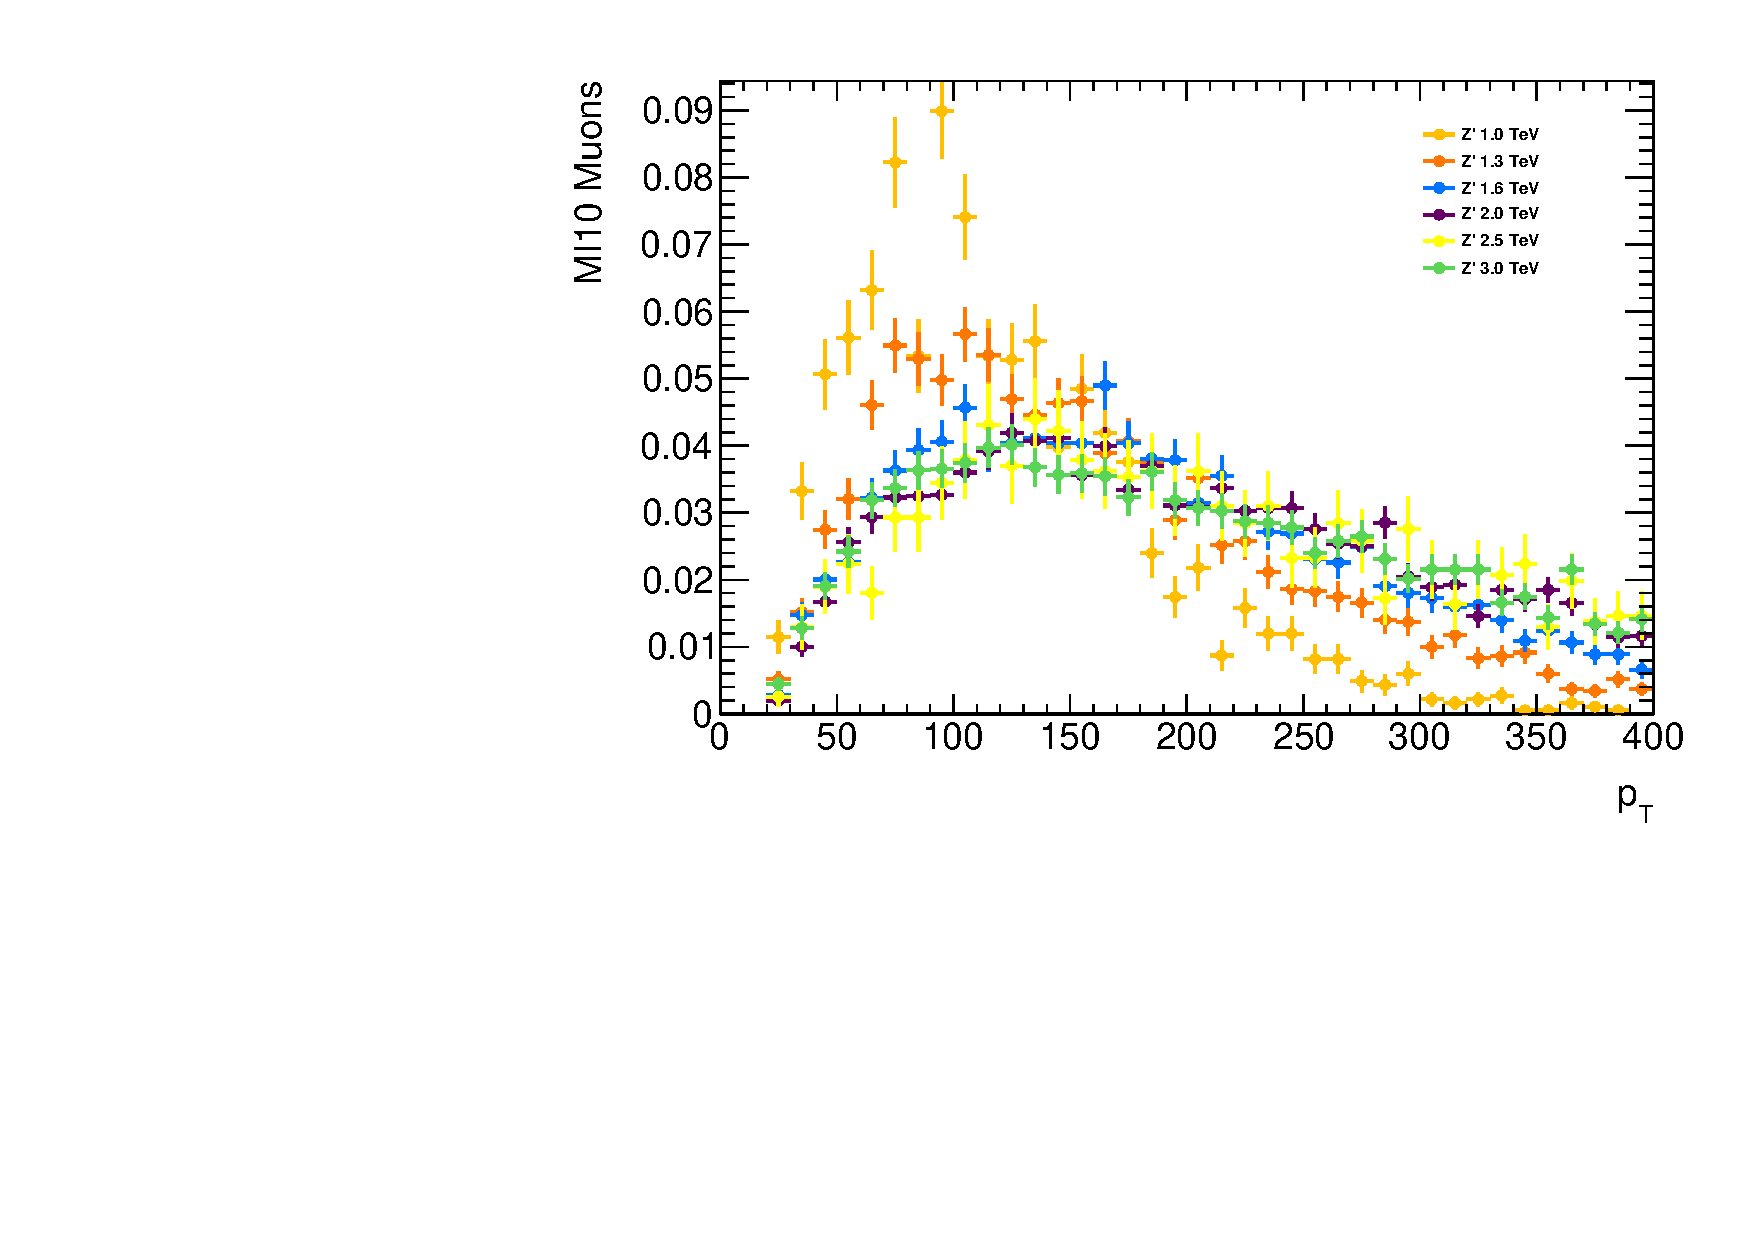
\includegraphics[width=\textwidth]{PartBoosted/Plots/h_mi10_pt.pdf}
\end{subfigure}
~
\begin{subfigure}{0.49\linewidth}
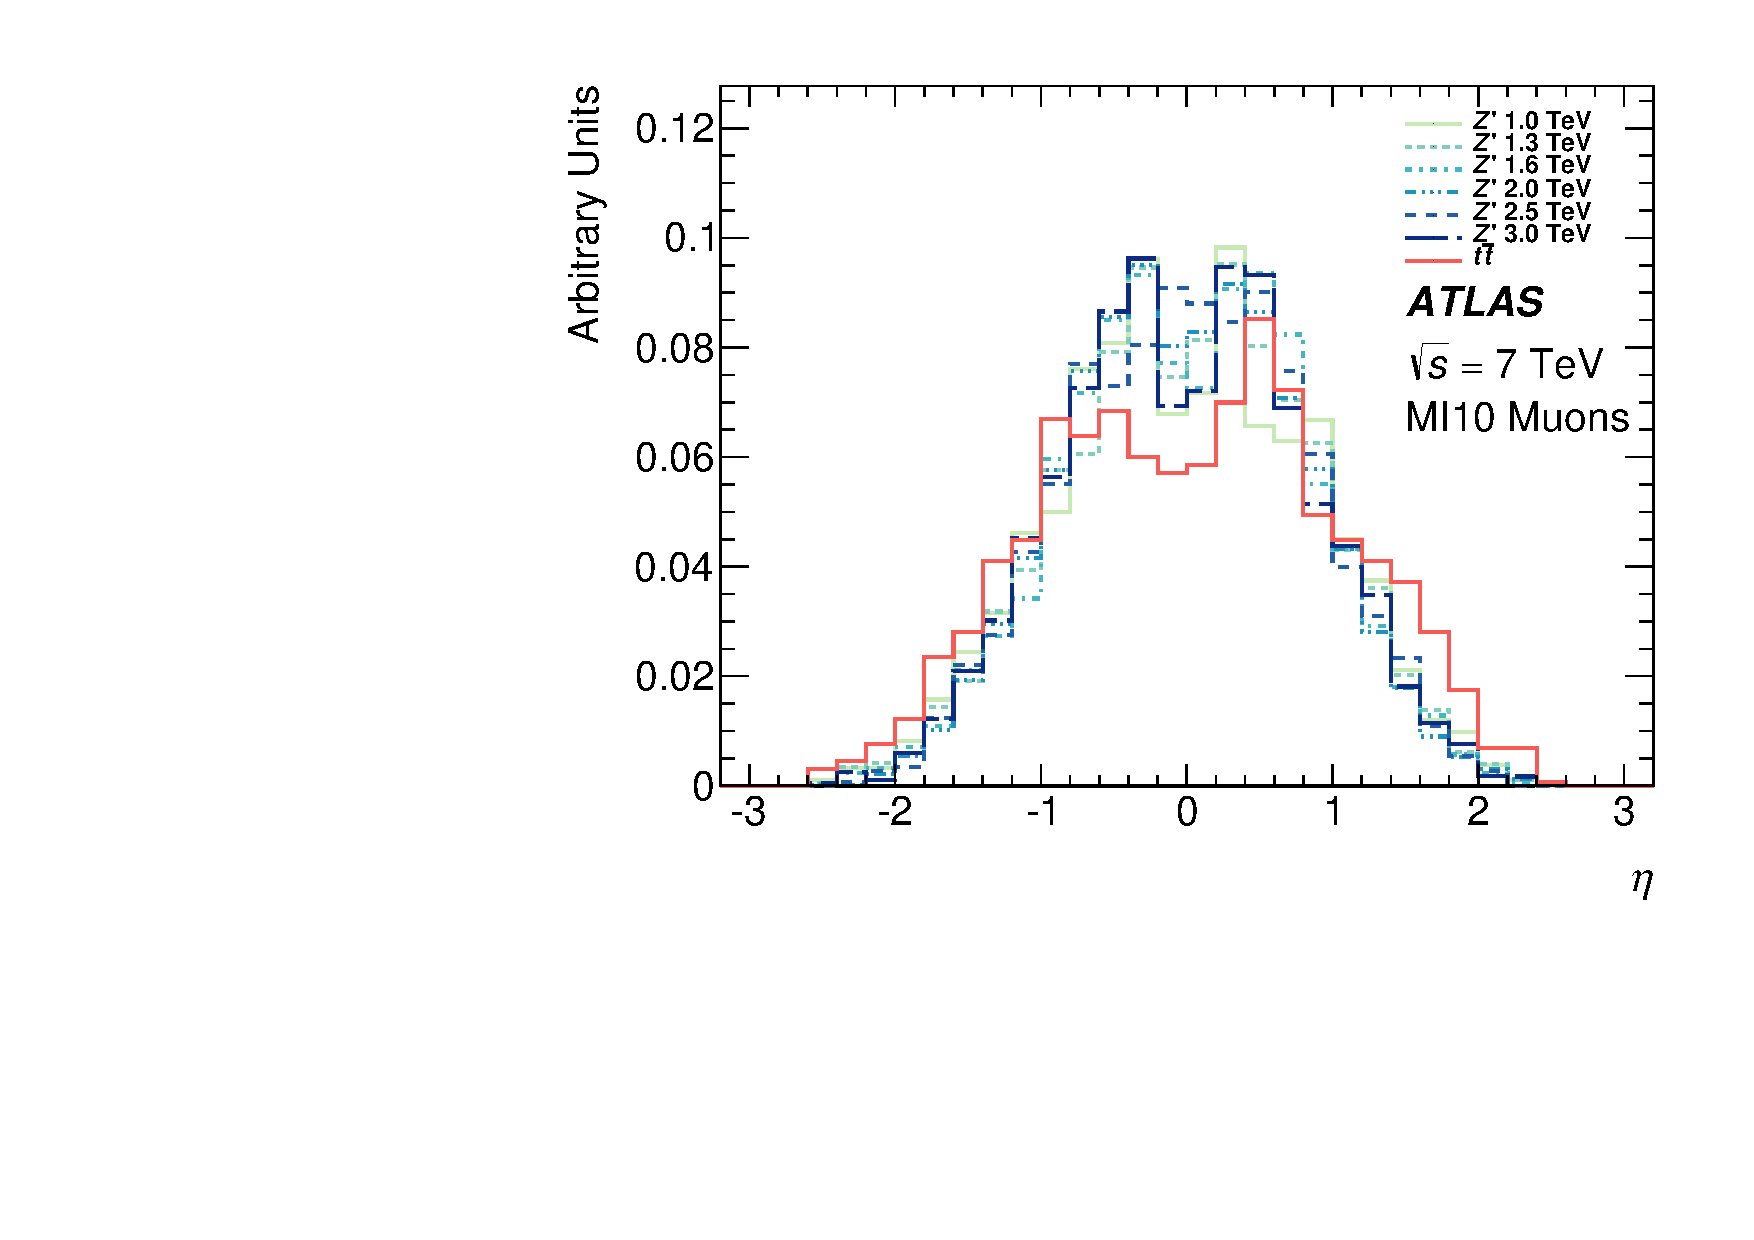
\includegraphics[width=\textwidth]{PartBoosted/Plots/h_mi10_eta.pdf}
\end{subfigure}

\begin{subfigure}{0.49\linewidth}
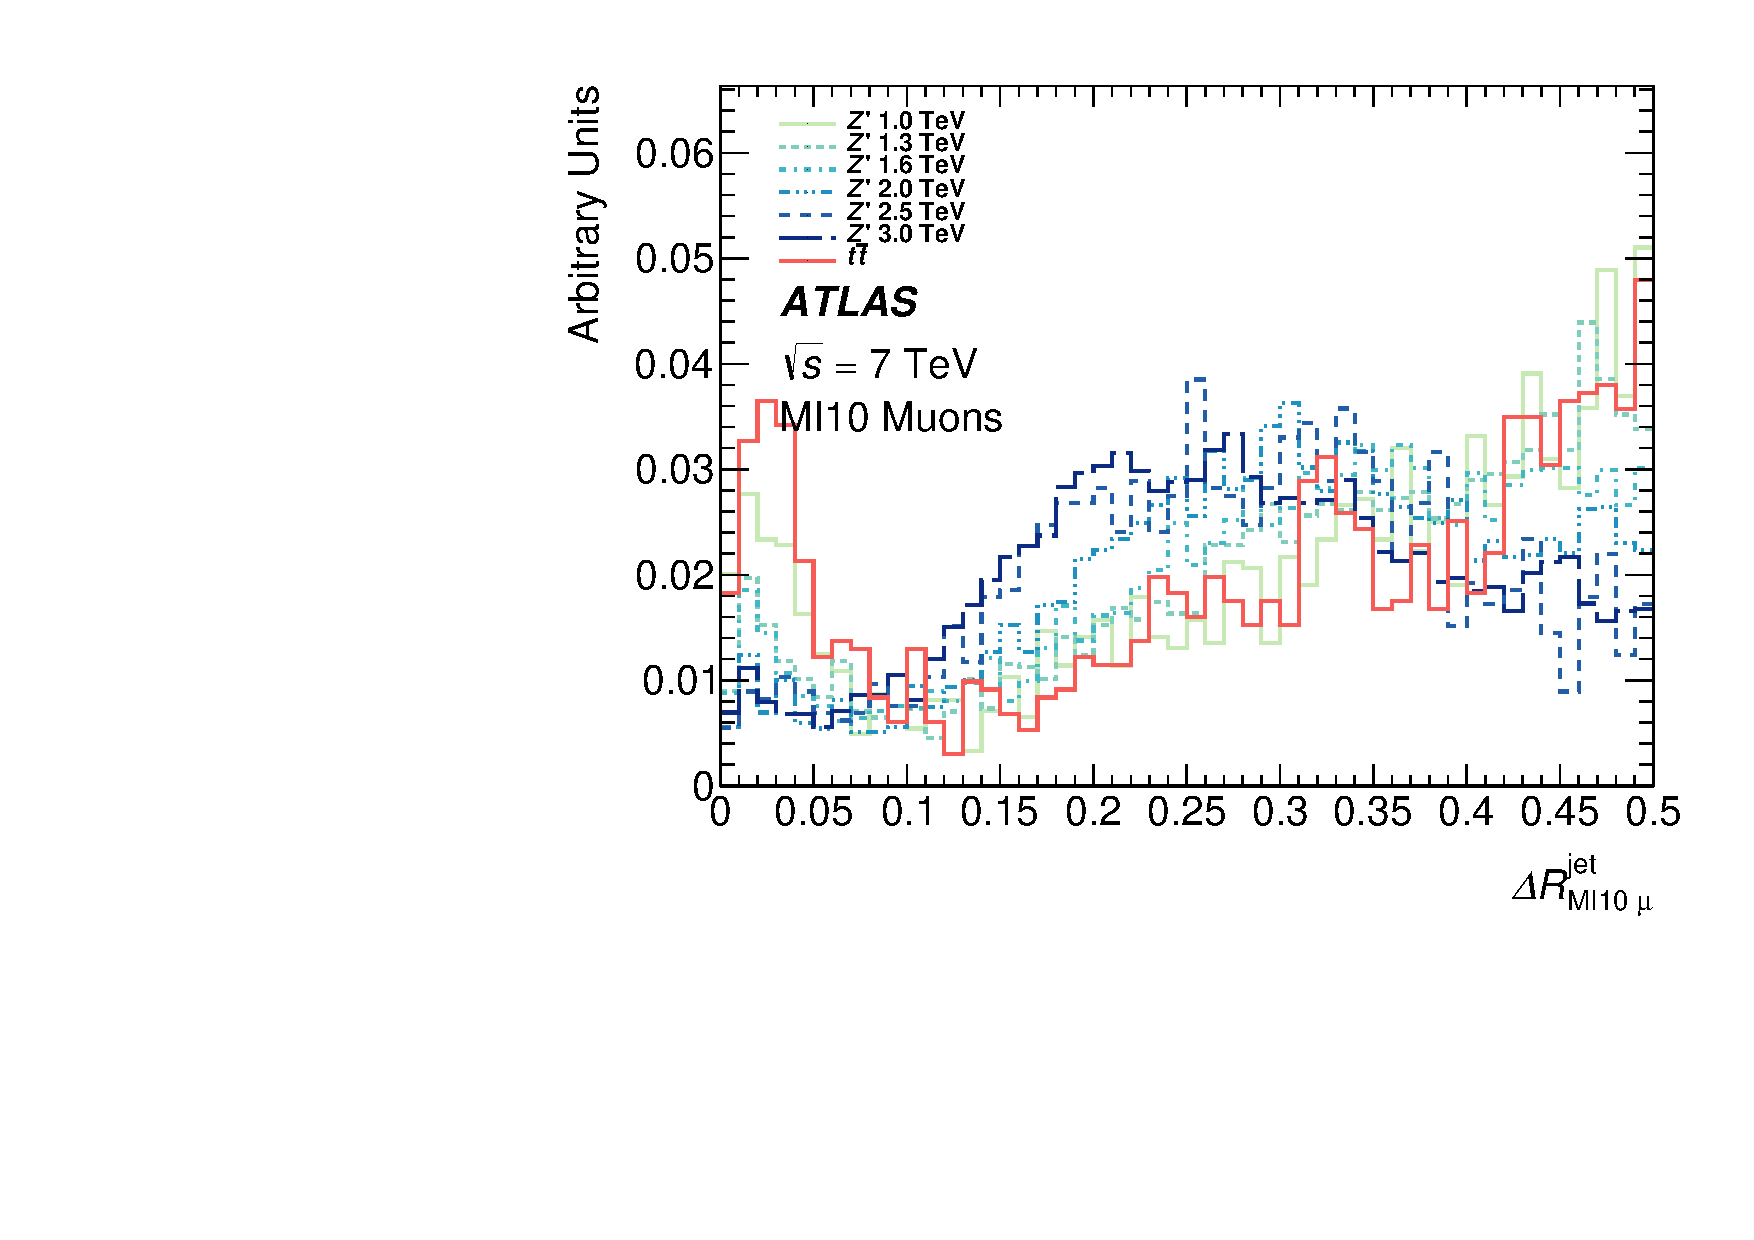
\includegraphics[width=\textwidth]{PartBoosted/Plots/h_mi10_jet_dr.pdf}
\end{subfigure}
~
\begin{subfigure}{0.49\linewidth}
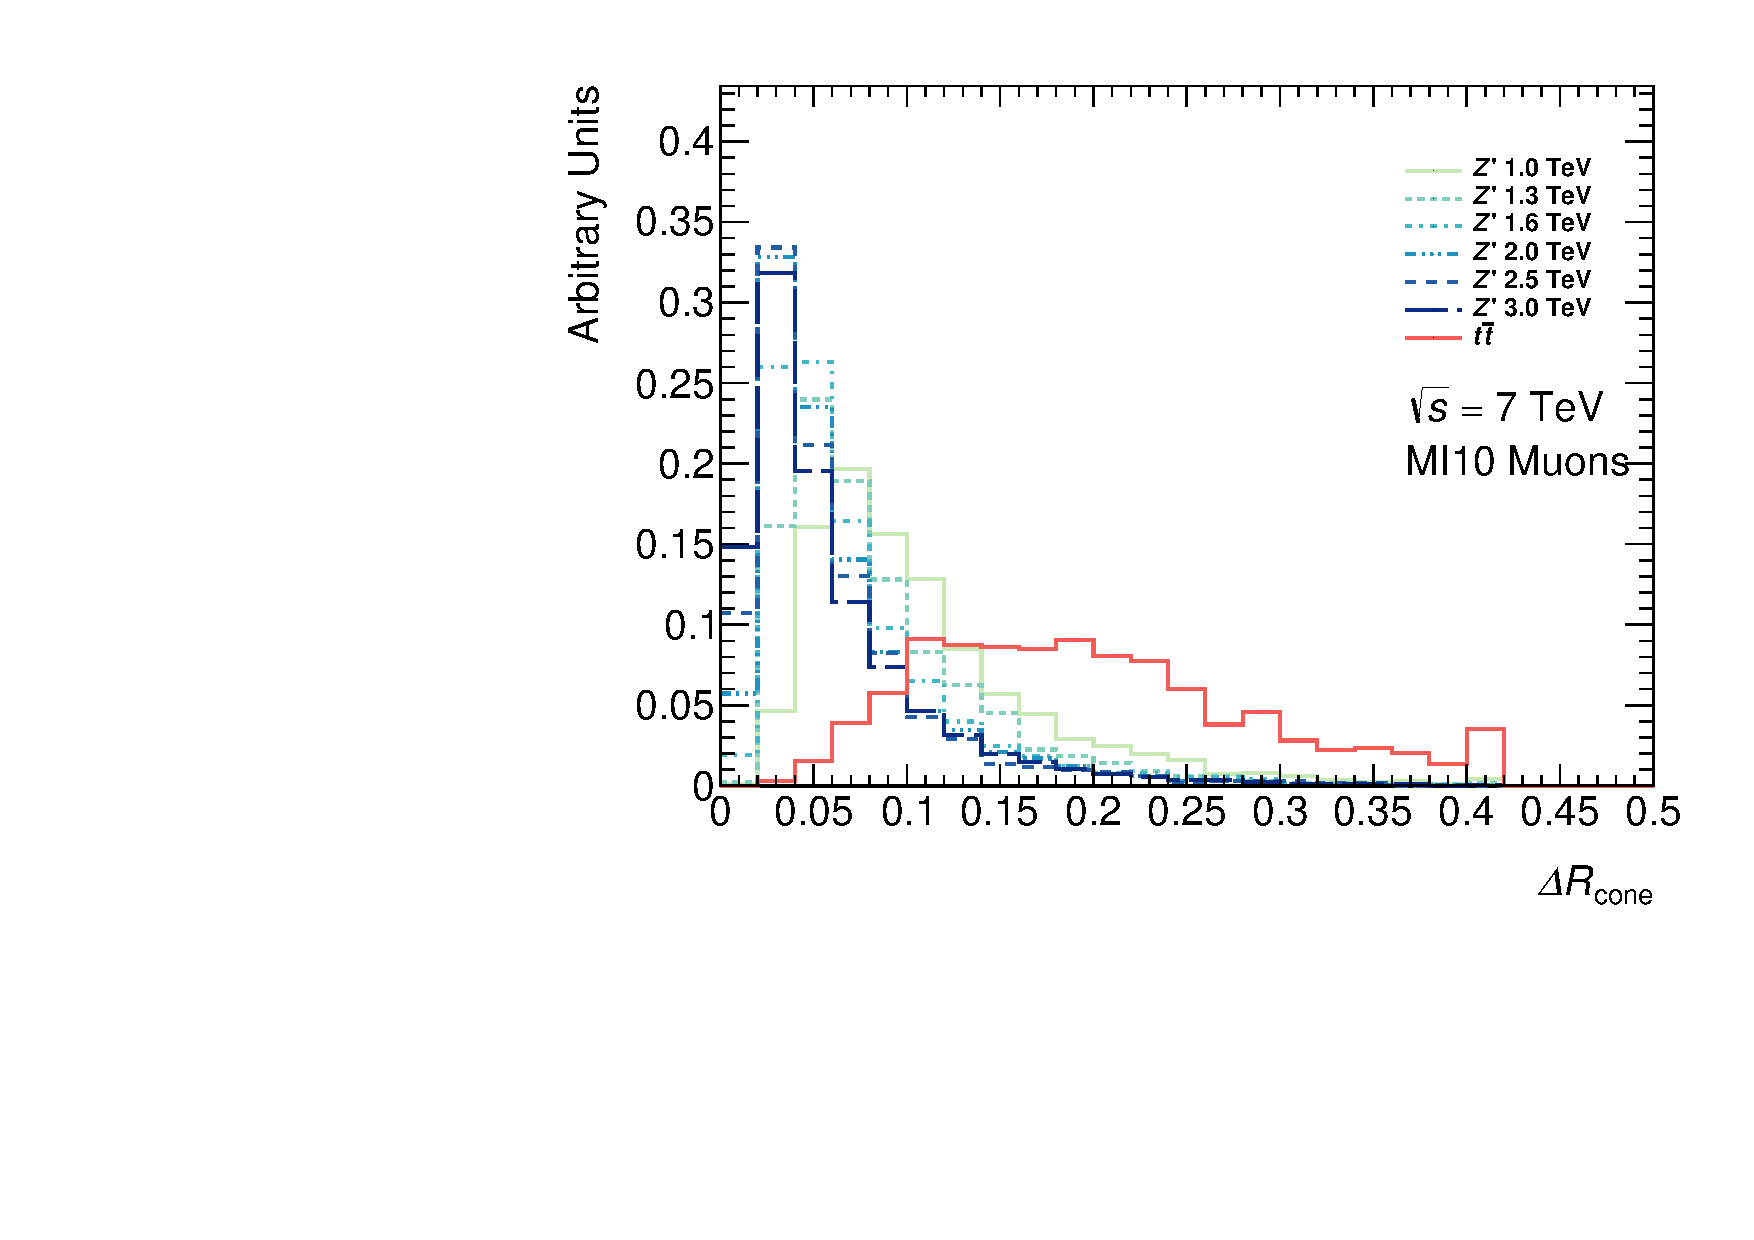
\includegraphics[width=\textwidth]{PartBoosted/Plots/h_mi10_coneSize.pdf}
\end{subfigure}

\caption{This figure shows the (a) transverse momentum and (b) pseudo-rapidity of muons which pass the MI10 selection, the (c) angular separation between those muons and the nearest jet in th event and (d) the cone size used in the selection for all tested \Zprime\ mass points.} \label{fig:BoostedControlSMT}
\end{figure}

The performance of both methodologies are then compared by measuring their efficiency.

\section{Efficiency definition} \label{sec:BoostedEfficiencyDefinition}

The efficiency measurement was designed to provide an accurate representation of the performance of the soft muon tagger and a valid comparison with mini-isolation. Additional sources of inefficiency such as muon reconstruction are separated out into an additional efficiency which is also quoted. See Fig.~\ref{fig:BoostedFlowChart} for a summary of the efficiency measurement.

\begin{figure}[t][th!]
  \centering
  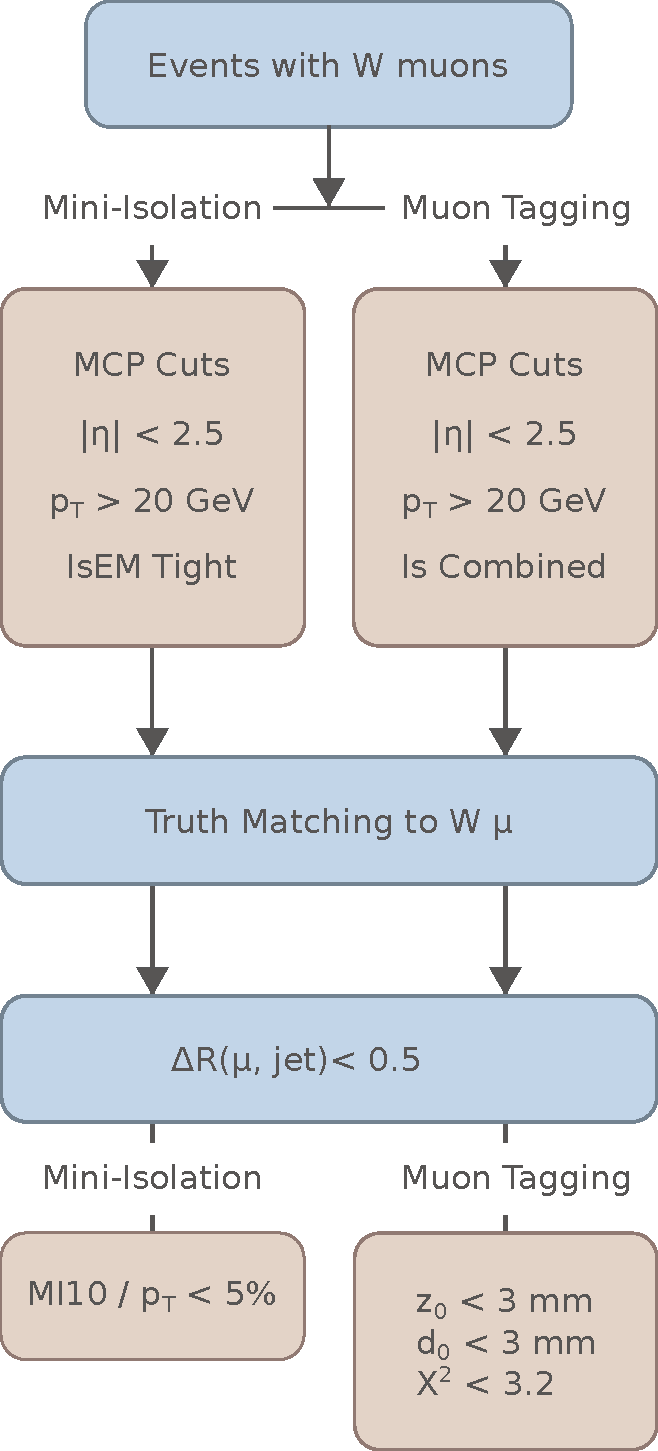
\includegraphics[width=0.45\textwidth]{PartBoosted/Plots/FlowChart.pdf}
  \caption{Structure of the efficiency measurement.} \label{fig:BoostedFlowChart}
\end{figure}

Firstly, events where a \W\ decays into a muon are selected, this becomes the pool of events from which the efficiency is measured. The selections then diverge and the two sets of reconstruction cuts described in Table~\ref{tab:BoostedReconstruction} are applied independently. The efficiency of each sets of reconstruction cuts are measured as:

\begin{equation*}
  \epsilon_{\textrm{reco}} = \frac{\textrm{Muons which pass selection}}{\textrm{All reconstructed muons}}
\end{equation*}

These good reconstructed muons are then truth-matched to the truth \m\ from the \W\ if the angular separate ($\Delta R$) between them is less than 0.01. This has an efficiency associated with it, defined as:

\begin{equation*}
  \epsilon_{\textrm{match}} = \frac{\textrm{Muons matched to truth \W\ muon}}{\textrm{Muons which pass selection}}
\end{equation*}

Note that at each stage the denominator is the numerator of the previous efficiency. This allows for a combination of all the efficiencies to obtain an inclusive measure which can used to approximate the number of \W\ muons which would be selected from collision data assuming that the simulation describes the data well.

Next the muons are required to be within $\Delta R < 0.5$ from a jet. The Muon Tagger requires that jets be near a jet, in addition the impetus behind the analysis is to probe highly boosted events exploiting the capabilities of \xsm\ tagging. This selection ensures that the muons available for \xsm\ tagging are indeed close to a jet. This selection also has an efficiency associated with it defined as:

\begin{equation*}
  \epsilon_{\textrm{non-iso}}=\frac{\textrm{Muons with $\Delta$R($\mu$, jet)$<$0.5}}{\textrm{Muons matched to truth \W\ muon}}
\end{equation*}

The final step is the application of both the mini-isolation selection and the muon tagging selection discussed a priori. These selections are associated with the final and most interesting sets of efficiencies, defined as:

\begin{equation*}
  \epsilon_{\textnormal{MT/MI10}} = \frac{\textnormal{Muons which pass MT/MI10 selection}}{\textnormal{Muons with $\Delta$R($\mu$, jet)$<$0.5}}
\end{equation*}

Please note that the denominator in every efficiency is a subset of the previous denominator. In other words each selection is applied in sequence and the efficiencies are calculated out of the remaining muons which passed the previous selection criteria.

Note that in the nominal analysis described in \cite{Boosted:ATLASExclusion7TeV} muons which are within $\Delta R$ of 0.1 of the jet would be removed. The impetus behind the analysis is to exploit the \xsm\ tagger to accept additional events where the signal muon emerges very close to the jet axis, thus overlap removal is not part of the \xsm\ tagging selection. In order to provide an accurate performance comparison between the \xsm\ tagger and mini-isolation, the overlap removal is applied only for the mini-isolation selection at the end of the chain. The additional acceptance gained by using \xsm\ tagger is compared to the mini-isolation selection with overlap included:

\begin{equation}
  \epsilon = \frac{\textrm{Muons that pass \xsm\ tagger - MI muons $\Delta$ R$<$0.1}}{\textrm{Total \W\ $\mu$}}
  \label{eq:BoostedAdditionalAcceptance}
\end{equation}

\section{Results}

Mini-isolation is a very efficient method for selecting muons. Table~\ref{tab:BoostedFinalEfficiencySummary} shows the efficiency for the \xsm\ tagger, mini-isolation and mini-isolation including overlap removal. Across the used mass range, the efficieny of selection remains above $80\%$ and in fact increases with a increased \Zprime\ mass. When the \Zprime\ has a mass of 3 TeV the efficiency of selection with mini-isolation is $92.5\%$ with no overlap removal. In contrast the efficiency of the \xsm\ tagger is more consistent across the used mass range and higher than mini-isolation for a given mass. For a \Zprime\ with a mass of 3 TeV the measured efficiency of the \xsm\ tagger is $96.2\%$. When applying the overlap removal the efficiency of mini-isolation falls to $85.0\%$.
As can be seen from Fig.~\ref{fig:BoostedEfficiencyVsDRmuj} the efficiency of mini-isolation dips for muons which are close to a jet however this occurs below the threshold of the overlap removal. Finally the additional acceptance gained as defined in \ref{eq:BoostedAdditionalAcceptance} is $4.03\%$. The additional acceptance gained in all mass points is also included in Table~\ref{tab:BoostedFinalEfficiencySummary}. 

\begin{table}
  \centering
  \begin{tabular}{|c|c|c|c|}
  \hline
  \Zprime\ Mass [TeV] & $\xsm$ & MI10 & MI10 + Overlap \tabularnewline
  \hline \hline
  1.0 & $94.9\%$ & $83.1\%$ & $67.0\%$ \tabularnewline
  1.3 & $95.8\%$ & $89.0\%$ & $79.2\%$ \tabularnewline
  1.6 & $95.9\%$ & $90.4\%$ & $81.9\%$ \tabularnewline
  2.0 & $96.0\%$ & $92.4\%$ & $85.7\%$ \tabularnewline
  2.5 & $95.8\%$ & $92.8\%$ & $85.1\%$ \tabularnewline
  3.0 & $96.2\%$ & $92.5\%$ & $85.0\%$ \tabularnewline
  \hline
  \end{tabular}
  \caption{Efficiency of selecting a muon by using the \xsm\ tagger against mini-isolation. Note that `MI10 + Overlap' is the efficiency of applying both the mini-isolation cut and overlap removal.}
  \label{tab:BoostedFinalEfficiencySummary}
\end{table}

\begin{figure}[t]
\begin{subfigure}{0.49\linewidth}
  \centering
  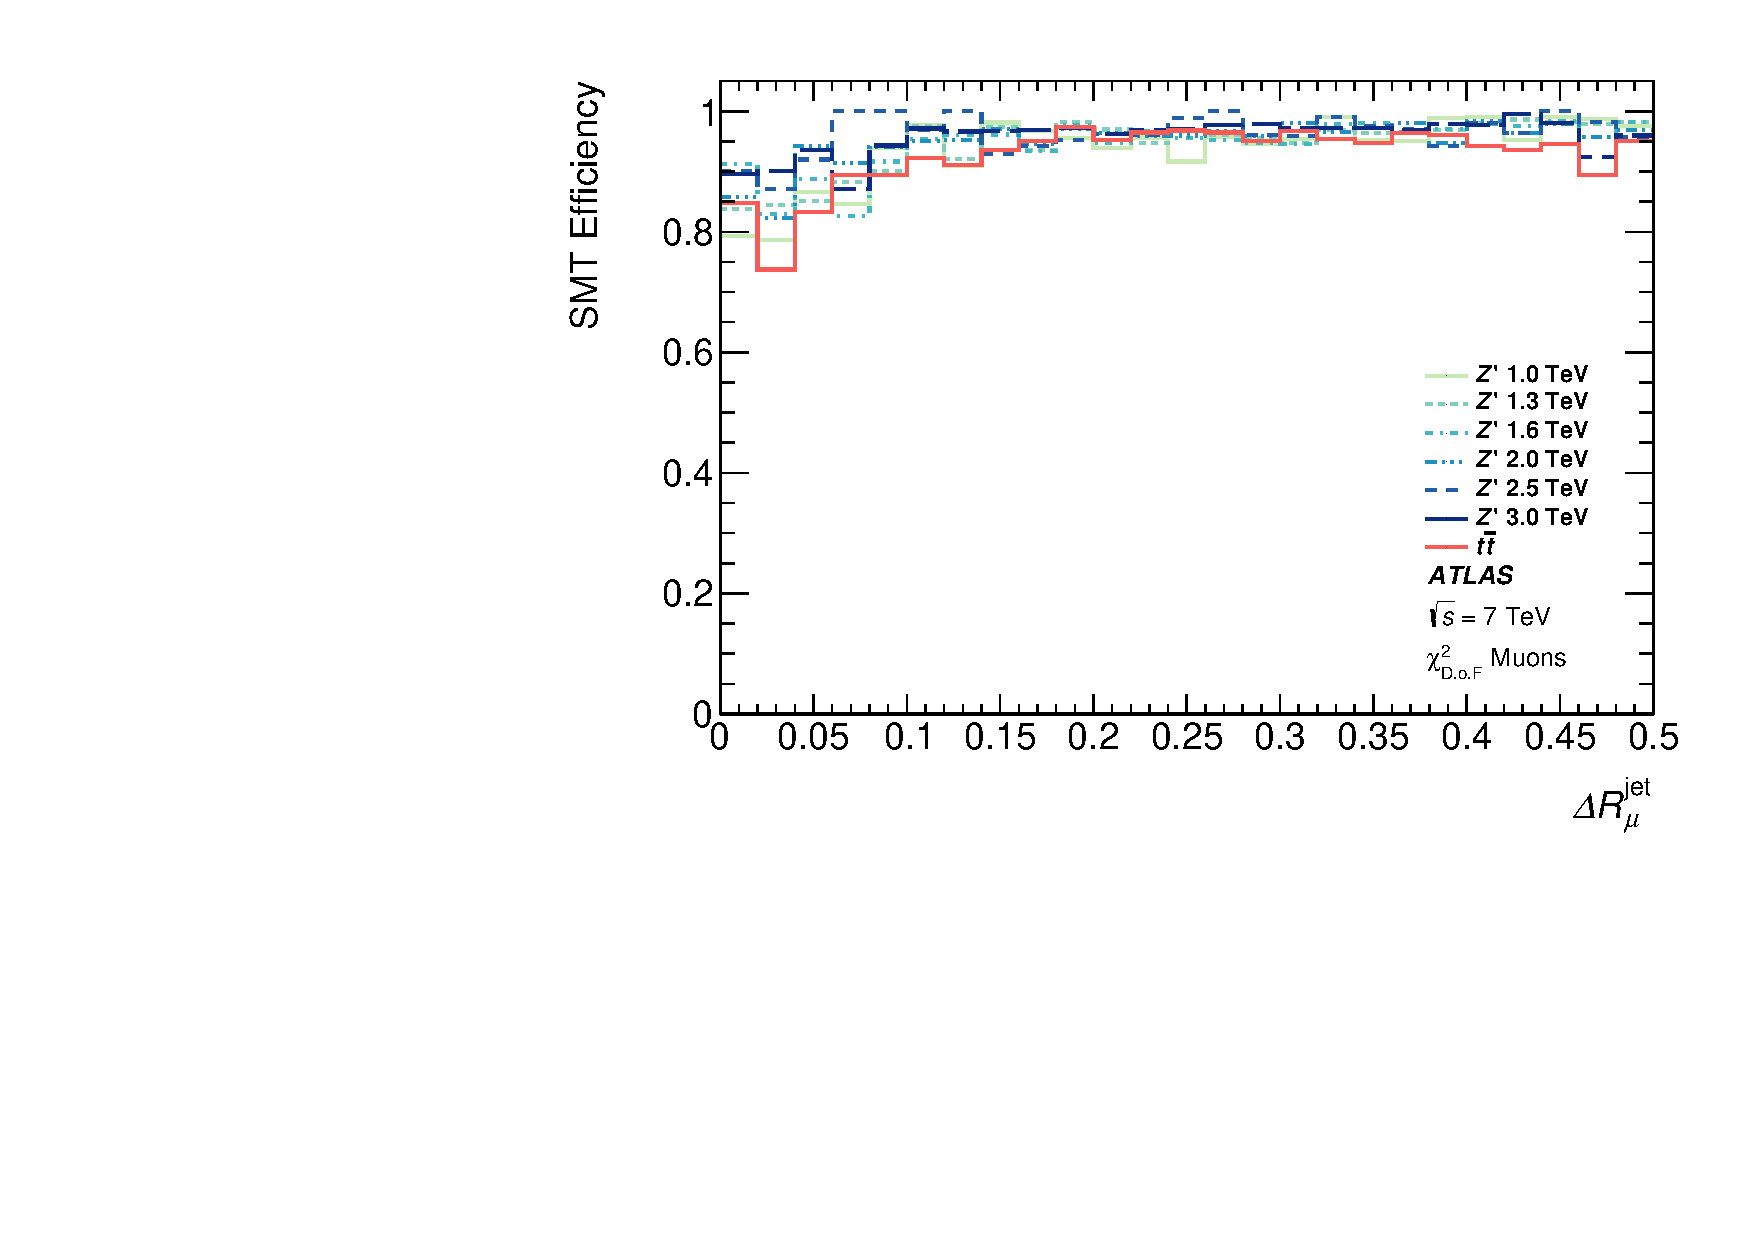
\includegraphics[width=\textwidth]{PartBoosted/Plots/he_staco_smt_dr.pdf}
  \caption{\xsm\ muon tagger} \label{fig:BoostedSMTeffVsDRmuj}
\end{subfigure}
~
\begin{subfigure}{0.49\linewidth}
  \centering
  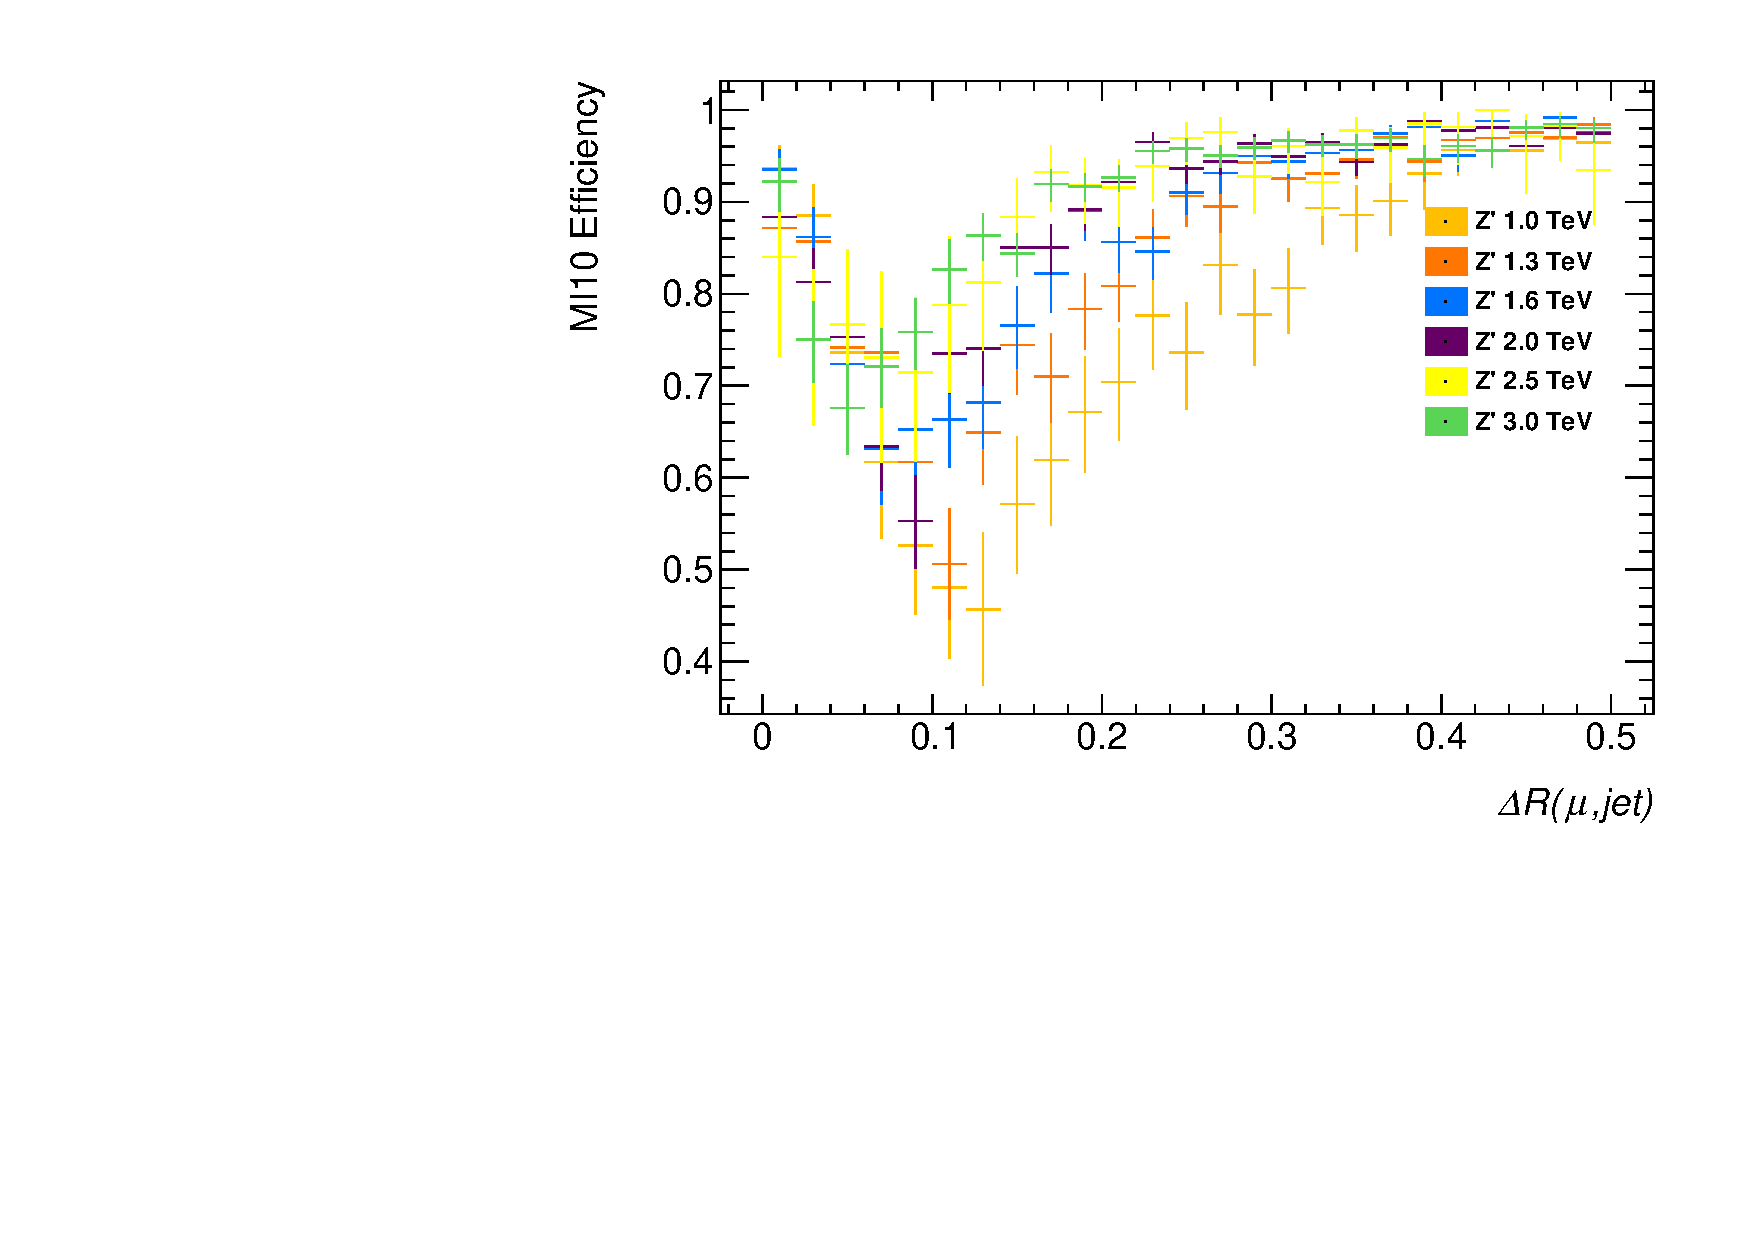
\includegraphics[width=\textwidth]{PartBoosted/Plots/he_muid_mi10_dr.pdf}
  \caption{Mini-isolation with $k_{T}=10$} \label{fig:BoostedMIeffVsDRmuj}
\end{subfigure}

\caption{Efficiency of mini-isolation ($k_{T}=10$) and \xsm muon tagger as a function of the angular separation between the reconstructed muon and the nearest reconstructed jet. Note the dip in the mini-isolation efficiency at low $\Delta R$. In the nominal analysis an overlap removal between the jet and the muon is applied.} \label{fig:BoostedEfficiencyVsDRmuj}
\end{figure}

\begin{figure}[t]
\begin{subfigure}{0.49\linewidth}\tabularnewline
  \centering
  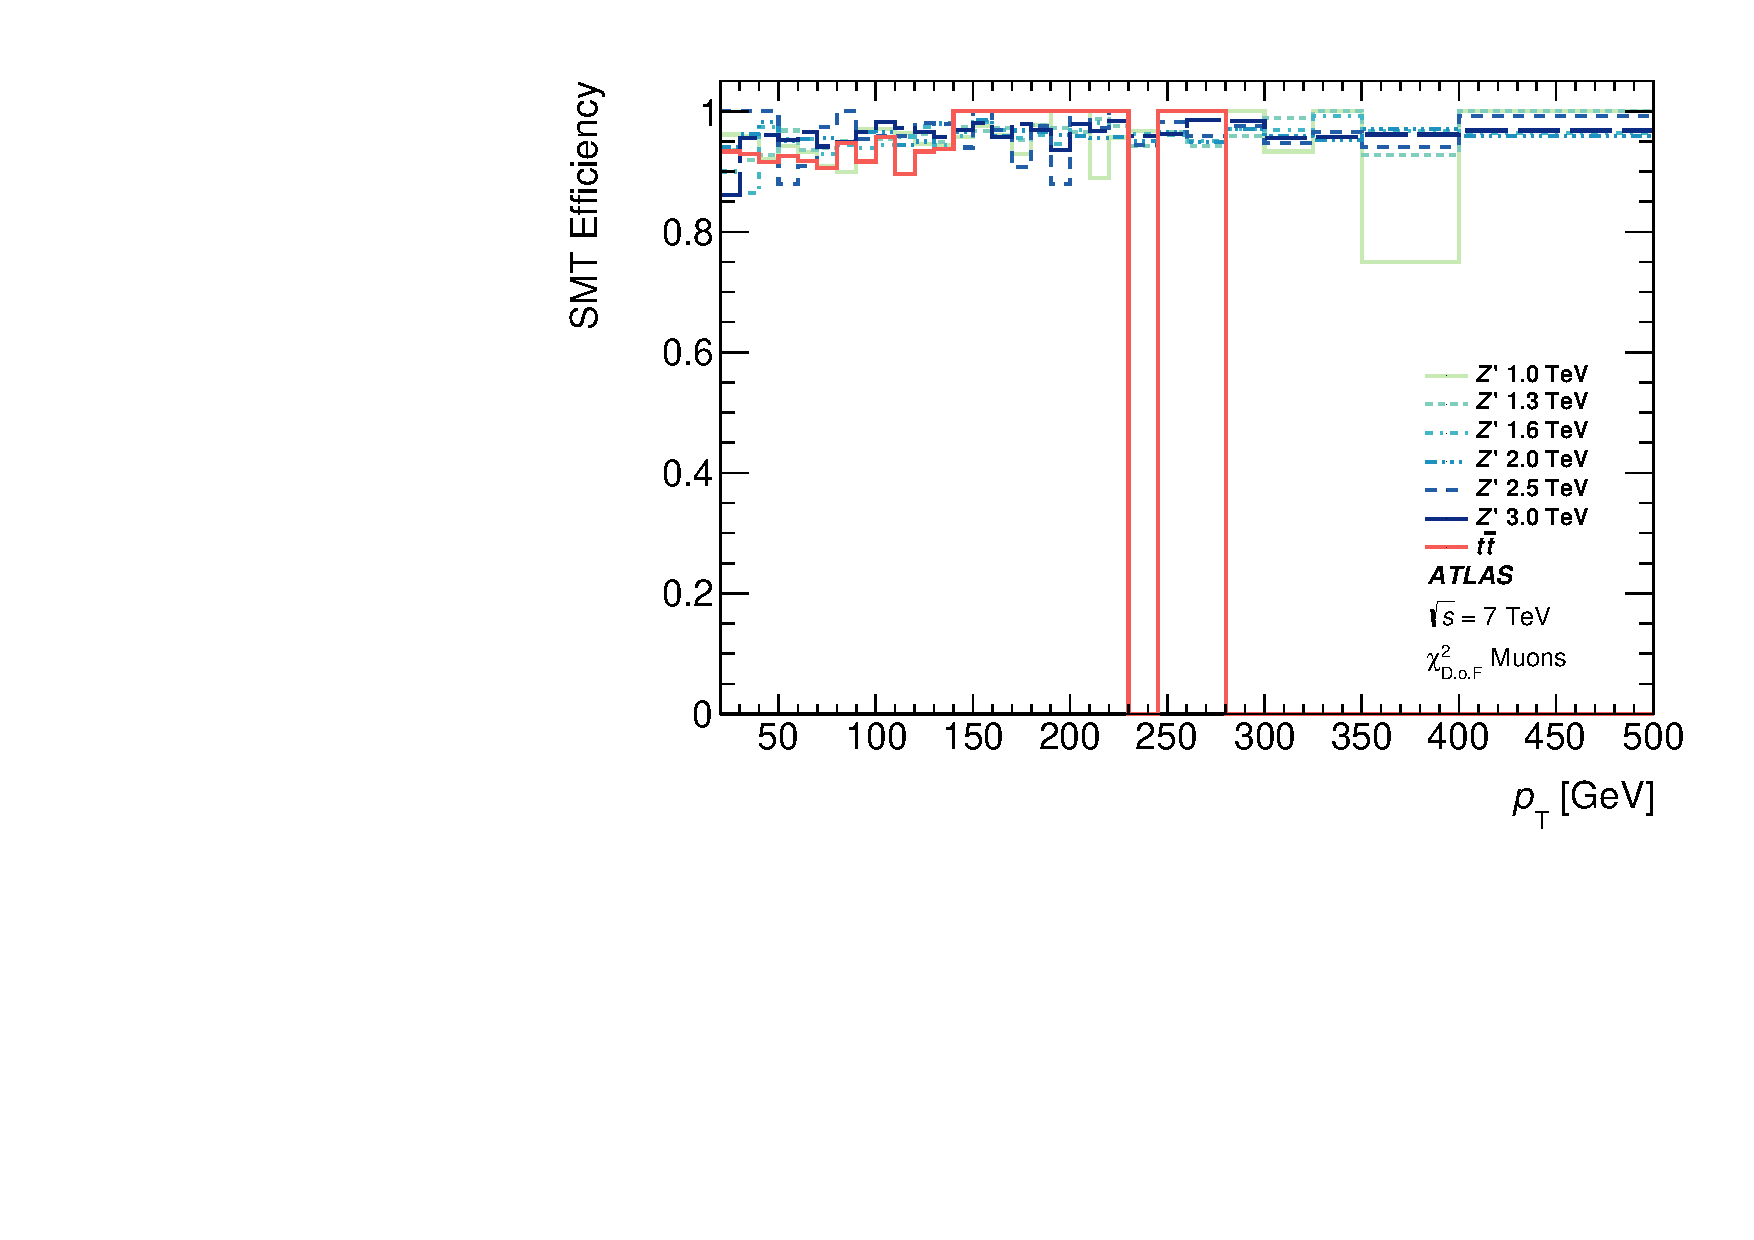
\includegraphics[width=\textwidth]{PartBoosted/Plots/he_staco_smt_pt.pdf}
  \caption{\xsm\ muon tagger} \label{fig:BoostedSMTeffVsPt}
\end{subfigure}
~
\begin{subfigure}{0.49\linewidth}
  \centering
  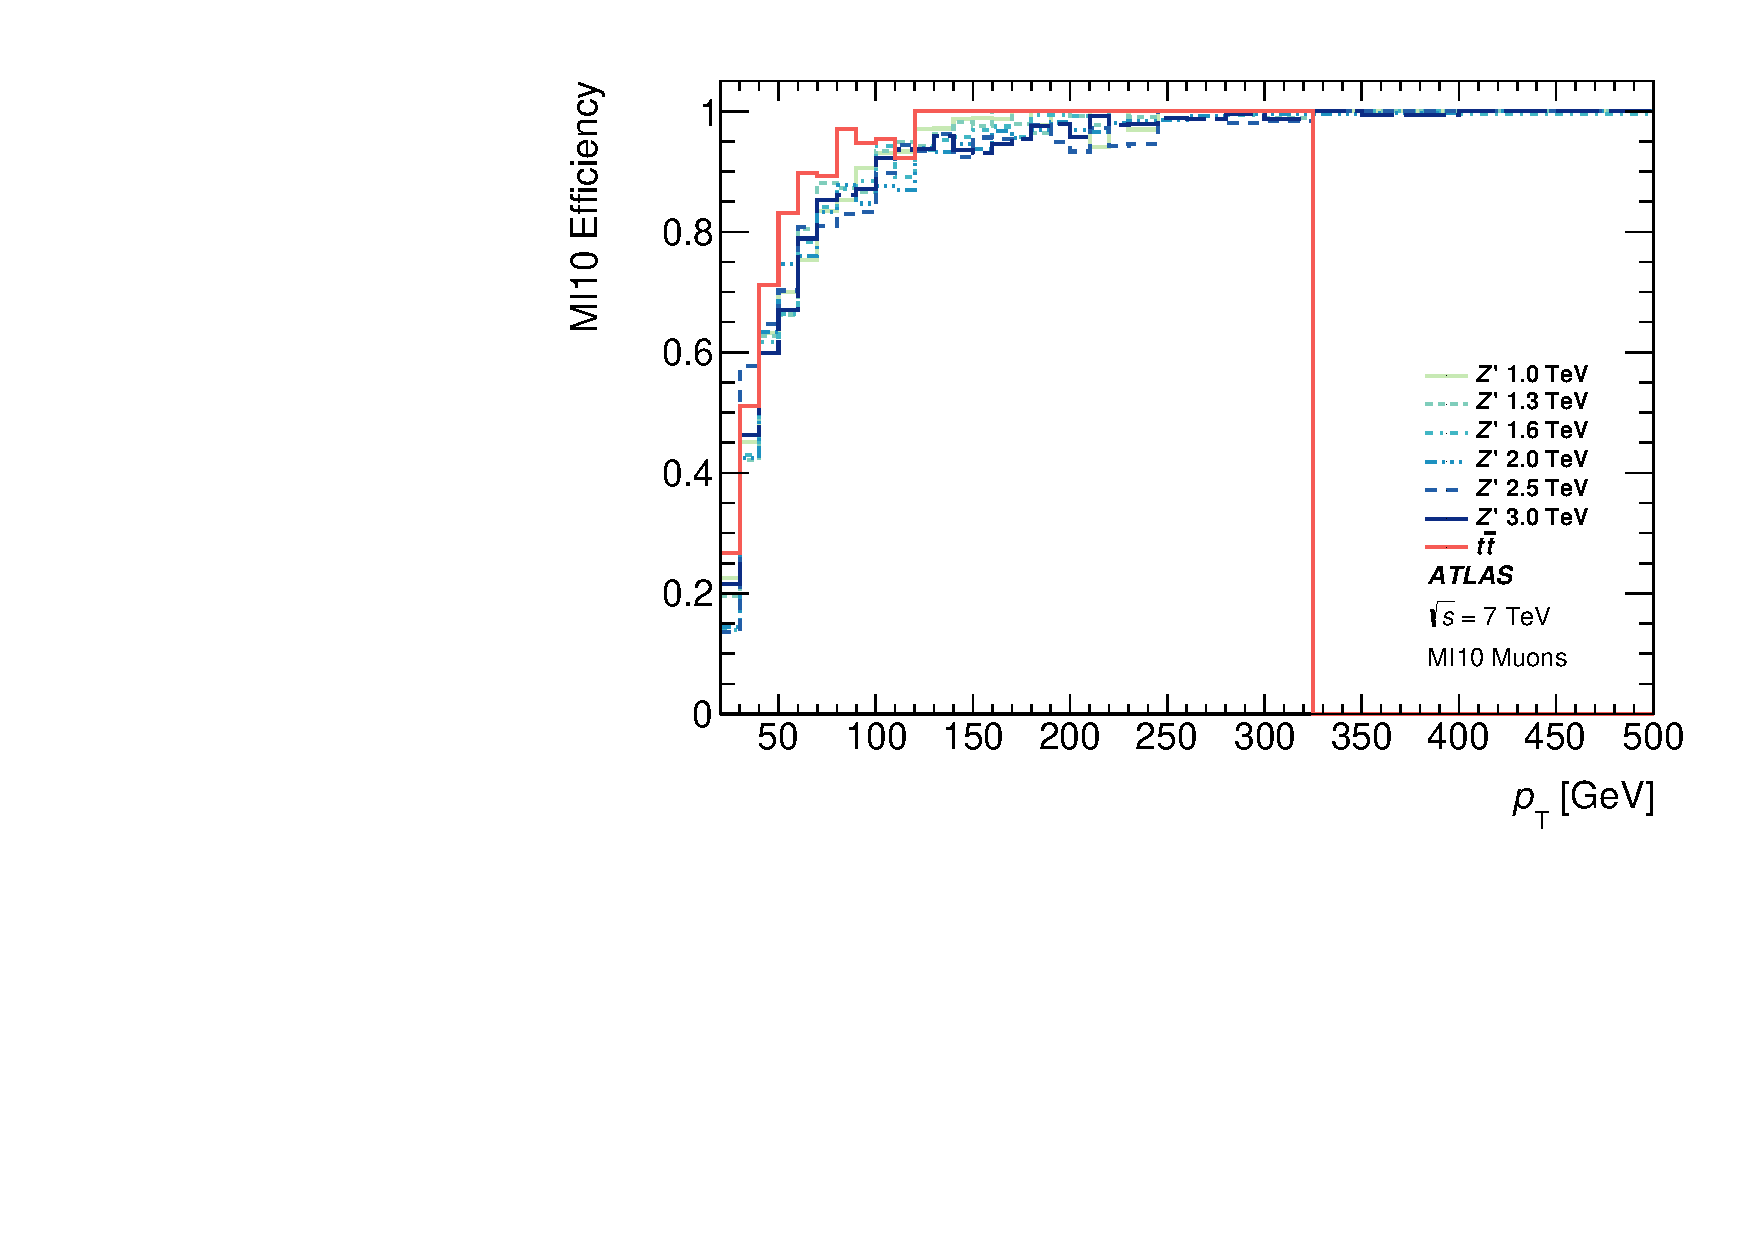
\includegraphics[width=\textwidth]{PartBoosted/Plots/he_muid_mi10_pt.pdf}
  \caption{Mini-isolation with $k_{T}=10$} \label{fig:BoostedMIeffVsPt}
\end{subfigure}

\caption{Efficiency of mini-isolation ($k_{T}=10$) and \xsm muon tagger as a function of the transverse momentum of the muon.} \label{fig:BoostedEfficiencyVsPt}
\end{figure}

\subsection{Background}

A preliminary examination of the amount of background was performed. This was done on the same sample of events but instead of selecting semileptonic events, the all-hadronic events are used as background. While these events do not perfectly mimic the true background, namely $b\bar{b}$, the lack of any real signal muons can provide a suitable preliminary substitute.

The lack of an isolation requirement is expected to result in a substantial increase in the amount of background selected. Additionally the semileptonic $b$-decays in $b\bar{b}$ would result in muons that the \xsm\ tagger will select. The analysis chain described in Section~\ref{sec:BoostedEfficiencyDefinition} is repeated on the same sample used a priori however the truth level selection of events with a \W\ muon is reversed, thus at truth level both \W\ bosons decay hadronically.

The results of this selection are presented in Table~\ref{tab:BoostedBackgroundResults}. As expected mini-isolation removes a substaintial amount of background while maintaining very high signal efficiency. In comparison, removing the isolation requirement greatly increases the background acceptance when using the \xsm\ tagger. A full treatment of the background would be required to account for the background present. 

The increase in signal acceptance does not make this methodology sufficiently advantageous particularly when considering the increase in fake rate. An examination of the $b$-tagging potential of the \xsm\ tagger is presented in the next section.

\begin{table}[!ht]
  \centering
  \caption{Fake rate of \xsm\ tagger, mini-isolation and mini-isolation including overlap removal as measured using all \Zprime\ mass points.}
  \label{tab:BoostedBackgroundResults}
  \begin{tabular}{|c|c|c|c|}
  \hline
  \Zprime\ Mass [TeV] & $\xsm$ & MI10 & MI10 + Overlap \tabularnewline
  \hline \hline
  1.0 & $92.8\%$ & $4.10\%$ & $2.39\%$ \tabularnewline
  1.3 & $92.4\%$ & $4.77\%$ & $3.66\%$ \tabularnewline
  1.6 & $91.8\%$ & $5.46\%$ & $4.55\%$ \tabularnewline
  2.0 & $91.1\%$ & $7.07\%$ & $6.09\%$ \tabularnewline
  2.5 & $90.0\%$ & $6.40\%$ & $5.57\%$ \tabularnewline
  3.0 & $90.1\%$ & $6.59\%$ & $5.68\%$ \tabularnewline
  \hline
  \end{tabular} 
\end{table}

\section{B-tagging potential in boosted events}

% Add some bullshit explanation of the methododly
% 

\begin{table}
  \caption{caption} \label{tab:BoostedBtaggingResults}
  \begin{tabular}{|c|c|c|c|c|}
      \hline
      \Zprime\ Mass [TeV] & Good Muons & Matched Muons & $\Delta R(\mu,jet)<0.5$ & \xsm-tagged \tabularnewline 
      \hline \hline
      1.0 & 16382 & 9807  ($59.8\%$) & 8722  ($88.9\%$) &  8237  ($94.4\%$) \tabularnewline 
      1.3 & 21099 & 13344 ($63.2\%$) & 12083 ($90.6\%$) &  11402 ($94.4\%$) \tabularnewline 
      1.6 & 19947 & 13012 ($65.2\%$) & 11929 ($91.7\%$) &  11240 ($94.2\%$) \tabularnewline 
      2.0 & 23391 & 15235 ($65.1\%$) & 14177 ($93.1\%$) &  13276 ($93.6\%$) \tabularnewline 
      2.5 & 5152  & 3347  ($64.9\%$) & 3137  ($93.7\%$) &  2922  ($93.1\%$) \tabularnewline 
      3.0 & 21766 & 13835 ($63.5\%$) & 13032 ($94.2\%$) &  12145 ($93.2\%$) \tabularnewline 
    \hline
  \end{tabular}
\end{table}
